
%% bare_jrnl_compsoc.tex
%% V1.4b
%% 2015/08/26
%% by Michael Shell
%% See:
%% http://www.michaelshell.org/
%% for current contact information.
%%
%% This is a skeleton file demonstrating the use of IEEEtran.cls
%% (requires IEEEtran.cls version 1.8b or later) with an IEEE
%% Computer Society journal paper.
%%
%% Support sites:
%% http://www.michaelshell.org/tex/ieeetran/
%% http://www.ctan.org/pkg/ieeetran
%% and
%% http://www.ieee.org/

%%*************************************************************************
%% Legal Notice:
%% This code is offered as-is without any warranty either expressed or
%% implied; without even the implied warranty of MERCHANTABILITY or
%% FITNESS FOR A PARTICULAR PURPOSE!
%% User assumes all risk.
%% In no event shall the IEEE or any contributor to this code be liable for
%% any damages or losses, including, but not limited to, incidental,
%% consequential, or any other damages, resulting from the use or misuse
%% of any information contained here.
%%
%% All comments are the opinions of their respective authors and are not
%% necessarily endorsed by the IEEE.
%%
%% This work is distributed under the LaTeX Project Public License (LPPL)
%% ( http://www.latex-project.org/ ) version 1.3, and may be freely used,
%% distributed and modified. A copy of the LPPL, version 1.3, is included
%% in the base LaTeX documentation of all distributions of LaTeX released
%% 2003/12/01 or later.
%% Retain all contribution notices and credits.
%% ** Modified files should be clearly indicated as such, including  **
%% ** renaming them and changing author support contact information. **
%%*************************************************************************


% *** Authors should verify (and, if needed, correct) their LaTeX system  ***
% *** with the testflow diagnostic prior to trusting their LaTeX platform ***
% *** with production work. The IEEE's font choices and paper sizes can   ***
% *** trigger bugs that do not appear when using other class files.       ***                          ***
% The testflow support page is at:
% http://www.michaelshell.org/tex/testflow/


\documentclass[10pt,journal,compsoc]{IEEEtran}
%
% If IEEEtran.cls has not been installed into the LaTeX system files,
% manually specify the path to it like:
% \documentclass[10pt,journal,compsoc]{../sty/IEEEtran}

\usepackage{textcomp}
\usepackage{hyperref}
\hypersetup{pdfpagemode=UseNone}
\usepackage{subfig}
\usepackage{booktabs}
\usepackage{multirow}
%\usepackage{natbib}
\usepackage{color,soul}
\usepackage{enumitem}
\usepackage{balance}
\usepackage{graphicx}
\usepackage[table]{xcolor}

%\usepackage{amsmath,scalerel}

%\DeclareMathOperator*{\Bigcdot}{\scalerel*{\cdot}{\bigodot}}

\newtheorem{cond}{Condition}
\newtheorem{defn}{Definition}

\usepackage{etoolbox}

\usepackage{microtype}

\usepackage{fixltx2e}

\usepackage{listings}

\definecolor{mygreen}{rgb}{0,0.6,0}
\definecolor{mygray}{rgb}{0.5,0.5,0.5}
\definecolor{mymauve}{rgb}{0.58,0,0.82}

\lstset{ %
  backgroundcolor=\color{white},   % choose the background color; you must add \usepackage{color} or \usepackage{xcolor}
  basicstyle=\ttfamily,% the size of the fonts that are used for the code
  breakatwhitespace=false,         % sets if automatic breaks should only happen at whitespace
  breaklines=true,                 % sets automatic line breaking
  captionpos=b,                    % sets the caption-position to bottom
  commentstyle=\color{mygreen},    % comment style
  deletekeywords={...},            % if you want to delete keywords from the given language
  escapeinside={\%*}{*)},          % if you want to add LaTeX within your code
  extendedchars=true,              % lets you use non-ASCII characters; for 8-bits encodings only, does not work with UTF-8
  frame=single,                    % adds a frame around the code
  keepspaces=true,                 % keeps spaces in text, useful for keeping indentation of code (possibly needs columns=flexible)
  keywordstyle=\color{blue},       % keyword style
  otherkeywords={module,bundle,design,port,connection,parameter},  %
  %keywords={pragma,unroll},       % if you want to add more keywords to the set keywords=[<number>]{<list of keywords>}
  %keywordstyle={[3]\color{red}},  % keyword style keywordstyle={[<number>]<style commands>},
  language=XML,                    % the language of the code
  numbers=left,                    % where to put the line-numbers; possible values are (none, left, right)
  numbersep=5pt,                   % how far the line-numbers are from the code
  numberstyle=\tiny\color{mygray}, % the style that is used for the line-numbers
  rulecolor=\color{black},         % if not set, the frame-color may be changed on line-breaks within not-black text (e.g. comments (green here))
  showspaces=false,                % show spaces everywhere adding particular underscores; it overrides 'showstringspaces'
  showstringspaces=false,          % underline spaces within strings only
  showtabs=false,                  % show tabs within strings adding particular underscores
  stepnumber=1,                    % the step between two line-numbers. If it's 1, each line will be numbered
  stringstyle=\color{mymauve},     % string literal style
  tabsize=2,                       % sets default tabsize to 2 spaces
  title=\lstname                   % show the filename of files included with \lstinputlisting; also try caption instead of title
}

%command to comment out stuff
\newcommand{\comment}[1]{}

%space saving!!!
\newcommand{\linespval}{1}
\comment{
\addtolength{\textfloatsep}{-10pt}
\addtolength{\floatsep}{-7pt}
\addtolength{\abovecaptionskip }{-5pt}
\addtolength{\dbltextfloatsep}{-7pt}
\addtolength{\dblfloatsep}{-5pt}

%Change caption size to small
\renewcommand{\captionfont}{\small}
\renewcommand{\captionlabelfont}{\small}

%reduce space between bib entries -- requires natbib
%\setlength{\bibsep}{0.04cm}

%use 0.95 or higher
\renewcommand{\linespval}{0.97}
\linespread{\linespval}

\setlist[itemize]{leftmargin=*}
\setlist[enumerate]{leftmargin=*}
}

\newcommand{\rtlbook}{\texttt{RTL2Booksim}}

\newcommand{\til}{{\fontfamily{ptm}\selectfont\texttildelow}}
\newcommand{\xx}{$\times${ }}


%shortcut command for pdf figures
\newcommand{\figvs}[4]{\begin{figure}[!t]
\centering
\includegraphics[width=#1\columnwidth,keepaspectratio,#3]{images/#2}
\caption{#4}
\label{#2}
\end{figure}}

%shortcut command for pdf figures
\newcommand{\figvsh}[4]{\begin{figure}[!h]
\centering
\includegraphics[width=#1\columnwidth,keepaspectratio,#3]{images/#2}
\caption{#4}
\label{#2}
\end{figure}}


%shortcut command for pdf figures
\newcommand{\figfull}[4]{\begin{figure*}[!t]
\centering
\includegraphics[width=#1\columnwidth,keepaspectratio,#3]{images/#2}
\caption{#4}
\label{#2}
\end{figure*}}


%adding subsubsubsection
\newcommand{\subsubsubsection}[1]{\vspace{0.2cm}\noindent\textbf{\textit{#1:}}}


% Some very useful LaTeX packages include:
% (uncomment the ones you want to load)


% *** MISC UTILITY PACKAGES ***
%
%\usepackage{ifpdf}
% Heiko Oberdiek's ifpdf.sty is very useful if you need conditional
% compilation based on whether the output is pdf or dvi.
% usage:
% \ifpdf
%   % pdf code
% \else
%   % dvi code
% \fi
% The latest version of ifpdf.sty can be obtained from:
% http://www.ctan.org/pkg/ifpdf
% Also, note that IEEEtran.cls V1.7 and later provides a builtin
% \ifCLASSINFOpdf conditional that works the same way.
% When switching from latex to pdflatex and vice-versa, the compiler may
% have to be run twice to clear warning/error messages.






% *** CITATION PACKAGES ***
%
\ifCLASSOPTIONcompsoc
  % IEEE Computer Society needs nocompress option
  % requires cite.sty v4.0 or later (November 2003)
  \usepackage[nocompress]{cite}
\else
  % normal IEEE
  \usepackage{cite}
\fi
% cite.sty was written by Donald Arseneau
% V1.6 and later of IEEEtran pre-defines the format of the cite.sty package
% \cite{} output to follow that of the IEEE. Loading the cite package will
% result in citation numbers being automatically sorted and properly
% "compressed/ranged". e.g., [1], [9], [2], [7], [5], [6] without using
% cite.sty will become [1], [2], [5]--[7], [9] using cite.sty. cite.sty's
% \cite will automatically add leading space, if needed. Use cite.sty's
% noadjust option (cite.sty V3.8 and later) if you want to turn this off
% such as if a citation ever needs to be enclosed in parenthesis.
% cite.sty is already installed on most LaTeX systems. Be sure and use
% version 5.0 (2009-03-20) and later if using hyperref.sty.
% The latest version can be obtained at:
% http://www.ctan.org/pkg/cite
% The documentation is contained in the cite.sty file itself.
%
% Note that some packages require special options to format as the Computer
% Society requires. In particular, Computer Society  papers do not use
% compressed citation ranges as is done in typical IEEE papers
% (e.g., [1]-[4]). Instead, they list every citation separately in order
% (e.g., [1], [2], [3], [4]). To get the latter we need to load the cite
% package with the nocompress option which is supported by cite.sty v4.0
% and later. Note also the use of a CLASSOPTION conditional provided by
% IEEEtran.cls V1.7 and later.





% *** GRAPHICS RELATED PACKAGES ***
%
\ifCLASSINFOpdf
  % \usepackage[pdftex]{graphicx}
  % declare the path(s) where your graphic files are
  % \graphicspath{{../pdf/}{../jpeg/}}
  % and their extensions so you won't have to specify these with
  % every instance of \includegraphics
  % \DeclareGraphicsExtensions{.pdf,.jpeg,.png}
\else
  % or other class option (dvipsone, dvipdf, if not using dvips). graphicx
  % will default to the driver specified in the system graphics.cfg if no
  % driver is specified.
  % \usepackage[dvips]{graphicx}
  % declare the path(s) where your graphic files are
  % \graphicspath{{../eps/}}
  % and their extensions so you won't have to specify these with
  % every instance of \includegraphics
  % \DeclareGraphicsExtensions{.eps}
\fi
% graphicx was written by David Carlisle and Sebastian Rahtz. It is
% required if you want graphics, photos, etc. graphicx.sty is already
% installed on most LaTeX systems. The latest version and documentation
% can be obtained at:
% http://www.ctan.org/pkg/graphicx
% Another good source of documentation is "Using Imported Graphics in
% LaTeX2e" by Keith Reckdahl which can be found at:
% http://www.ctan.org/pkg/epslatex
%
% latex, and pdflatex in dvi mode, support graphics in encapsulated
% postscript (.eps) format. pdflatex in pdf mode supports graphics
% in .pdf, .jpeg, .png and .mps (metapost) formats. Users should ensure
% that all non-photo figures use a vector format (.eps, .pdf, .mps) and
% not a bitmapped formats (.jpeg, .png). The IEEE frowns on bitmapped formats
% which can result in "jaggedy"/blurry rendering of lines and letters as
% well as large increases in file sizes.
%
% You can find documentation about the pdfTeX application at:
% http://www.tug.org/applications/pdftex






% *** MATH PACKAGES ***
%
%\usepackage{amsmath}
% A popular package from the American Mathematical Society that provides
% many useful and powerful commands for dealing with mathematics.
%
% Note that the amsmath package sets \interdisplaylinepenalty to 10000
% thus preventing page breaks from occurring within multiline equations. Use:
%\interdisplaylinepenalty=2500
% after loading amsmath to restore such page breaks as IEEEtran.cls normally
% does. amsmath.sty is already installed on most LaTeX systems. The latest
% version and documentation can be obtained at:
% http://www.ctan.org/pkg/amsmath





% *** SPECIALIZED LIST PACKAGES ***
%
%\usepackage{algorithmic}
% algorithmic.sty was written by Peter Williams and Rogerio Brito.
% This package provides an algorithmic environment fo describing algorithms.
% You can use the algorithmic environment in-text or within a figure
% environment to provide for a floating algorithm. Do NOT use the algorithm
% floating environment provided by algorithm.sty (by the same authors) or
% algorithm2e.sty (by Christophe Fiorio) as the IEEE does not use dedicated
% algorithm float types and packages that provide these will not provide
% correct IEEE style captions. The latest version and documentation of
% algorithmic.sty can be obtained at:
% http://www.ctan.org/pkg/algorithms
% Also of interest may be the (relatively newer and more customizable)
% algorithmicx.sty package by Szasz Janos:
% http://www.ctan.org/pkg/algorithmicx




% *** ALIGNMENT PACKAGES ***
%
%\usepackage{array}
% Frank Mittelbach's and David Carlisle's array.sty patches and improves
% the standard LaTeX2e array and tabular environments to provide better
% appearance and additional user controls. As the default LaTeX2e table
% generation code is lacking to the point of almost being broken with
% respect to the quality of the end results, all users are strongly
% advised to use an enhanced (at the very least that provided by array.sty)
% set of table tools. array.sty is already installed on most systems. The
% latest version and documentation can be obtained at:
% http://www.ctan.org/pkg/array


% IEEEtran contains the IEEEeqnarray family of commands that can be used to
% generate multiline equations as well as matrices, tables, etc., of high
% quality.




% *** SUBFIGURE PACKAGES ***
%\ifCLASSOPTIONcompsoc
%  \usepackage[caption=false,font=footnotesize,labelfont=sf,textfont=sf]{subfig}
%\else
%  \usepackage[caption=false,font=footnotesize]{subfig}
%\fi
% subfig.sty, written by Steven Douglas Cochran, is the modern replacement
% for subfigure.sty, the latter of which is no longer maintained and is
% incompatible with some LaTeX packages including fixltx2e. However,
% subfig.sty requires and automatically loads Axel Sommerfeldt's caption.sty
% which will override IEEEtran.cls' handling of captions and this will result
% in non-IEEE style figure/table captions. To prevent this problem, be sure
% and invoke subfig.sty's "caption=false" package option (available since
% subfig.sty version 1.3, 2005/06/28) as this is will preserve IEEEtran.cls
% handling of captions.
% Note that the Computer Society format requires a sans serif font rather
% than the serif font used in traditional IEEE formatting and thus the need
% to invoke different subfig.sty package options depending on whether
% compsoc mode has been enabled.
%
% The latest version and documentation of subfig.sty can be obtained at:
% http://www.ctan.org/pkg/subfig




% *** FLOAT PACKAGES ***
%
%\usepackage{fixltx2e}
% fixltx2e, the successor to the earlier fix2col.sty, was written by
% Frank Mittelbach and David Carlisle. This package corrects a few problems
% in the LaTeX2e kernel, the most notable of which is that in current
% LaTeX2e releases, the ordering of single and double column floats is not
% guaranteed to be preserved. Thus, an unpatched LaTeX2e can allow a
% single column figure to be placed prior to an earlier double column
% figure.
% Be aware that LaTeX2e kernels dated 2015 and later have fixltx2e.sty's
% corrections already built into the system in which case a warning will
% be issued if an attempt is made to load fixltx2e.sty as it is no longer
% needed.
% The latest version and documentation can be found at:
% http://www.ctan.org/pkg/fixltx2e


%\usepackage{stfloats}
% stfloats.sty was written by Sigitas Tolusis. This package gives LaTeX2e
% the ability to do double column floats at the bottom of the page as well
% as the top. (e.g., "\begin{figure*}[!b]" is not normally possible in
% LaTeX2e). It also provides a command:
%\fnbelowfloat
% to enable the placement of footnotes below bottom floats (the standard
% LaTeX2e kernel puts them above bottom floats). This is an invasive package
% which rewrites many portions of the LaTeX2e float routines. It may not work
% with other packages that modify the LaTeX2e float routines. The latest
% version and documentation can be obtained at:
% http://www.ctan.org/pkg/stfloats
% Do not use the stfloats baselinefloat ability as the IEEE does not allow
% \baselineskip to stretch. Authors submitting work to the IEEE should note
% that the IEEE rarely uses double column equations and that authors should try
% to avoid such use. Do not be tempted to use the cuted.sty or midfloat.sty
% packages (also by Sigitas Tolusis) as the IEEE does not format its papers in
% such ways.
% Do not attempt to use stfloats with fixltx2e as they are incompatible.
% Instead, use Morten Hogholm'a dblfloatfix which combines the features
% of both fixltx2e and stfloats:
%
% \usepackage{dblfloatfix}
% The latest version can be found at:
% http://www.ctan.org/pkg/dblfloatfix




%\ifCLASSOPTIONcaptionsoff
%  \usepackage[nomarkers]{endfloat}
% \let\MYoriglatexcaption\caption
% \renewcommand{\caption}[2][\relax]{\MYoriglatexcaption[#2]{#2}}
%\fi
% endfloat.sty was written by James Darrell McCauley, Jeff Goldberg and
% Axel Sommerfeldt. This package may be useful when used in conjunction with
% IEEEtran.cls'  captionsoff option. Some IEEE journals/societies require that
% submissions have lists of figures/tables at the end of the paper and that
% figures/tables without any captions are placed on a page by themselves at
% the end of the document. If needed, the draftcls IEEEtran class option or
% \CLASSINPUTbaselinestretch interface can be used to increase the line
% spacing as well. Be sure and use the nomarkers option of endfloat to
% prevent endfloat from "marking" where the figures would have been placed
% in the text. The two hack lines of code above are a slight modification of
% that suggested by in the endfloat docs (section 8.4.1) to ensure that
% the full captions always appear in the list of figures/tables - even if
% the user used the short optional argument of \caption[]{}.
% IEEE papers do not typically make use of \caption[]'s optional argument,
% so this should not be an issue. A similar trick can be used to disable
% captions of packages such as subfig.sty that lack options to turn off
% the subcaptions:
% For subfig.sty:
% \let\MYorigsubfloat\subfloat
% \renewcommand{\subfloat}[2][\relax]{\MYorigsubfloat[]{#2}}
% However, the above trick will not work if both optional arguments of
% the \subfloat command are used. Furthermore, there needs to be a
% description of each subfigure *somewhere* and endfloat does not add
% subfigure captions to its list of figures. Thus, the best approach is to
% avoid the use of subfigure captions (many IEEE journals avoid them anyway)
% and instead reference/explain all the subfigures within the main caption.
% The latest version of endfloat.sty and its documentation can obtained at:
% http://www.ctan.org/pkg/endfloat
%
% The IEEEtran \ifCLASSOPTIONcaptionsoff conditional can also be used
% later in the document, say, to conditionally put the References on a
% page by themselves.




% *** PDF, URL AND HYPERLINK PACKAGES ***
%
%\usepackage{url}
% url.sty was written by Donald Arseneau. It provides better support for
% handling and breaking URLs. url.sty is already installed on most LaTeX
% systems. The latest version and documentation can be obtained at:
% http://www.ctan.org/pkg/url
% Basically, \url{my_url_here}.





% *** Do not adjust lengths that control margins, column widths, etc. ***
% *** Do not use packages that alter fonts (such as pslatex).         ***
% There should be no need to do such things with IEEEtran.cls V1.6 and later.
% (Unless specifically asked to do so by the journal or conference you plan
% to submit to, of course. )


% correct bad hyphenation here
\hyphenation{op-tical net-works semi-conduc-tor}


\begin{document}

%
% paper title
% Titles are generally capitalized except for words such as a, an, and, as,
% at, but, by, for, in, nor, of, on, or, the, to and up, which are usually
% not capitalized unless they are the first or last word of the title.
% Linebreaks \\ can be used within to get better formatting as desired.
% Do not put math or special symbols in the title.
%\title{Design and Applications for Embedded Networks-on-Chip on Field-Programmable Gate-Arrays}
\title{Design and Applications for Embedded Networks-on-Chip on FPGAs}
%
%
% author names and IEEE memberships
% note positions of commas and nonbreaking spaces ( ~ ) LaTeX will not break
% a structure at a ~ so this keeps an author's name from being broken across
% two lines.
% use \thanks{} to gain access to the first footnote area
% a separate \thanks must be used for each paragraph as LaTeX2e's \thanks
% was not built to handle multiple paragraphs
%
%
%\IEEEcompsocitemizethanks is a special \thanks that produces the bulleted
% lists the Computer Society journals use for "first footnote" author
% affiliations. Use \IEEEcompsocthanksitem which works much like \item
% for each affiliation group. When not in compsoc mode,
% \IEEEcompsocitemizethanks becomes like \thanks and
% \IEEEcompsocthanksitem becomes a line break with idention. This
% facilitates dual compilation, although admittedly the differences in the
% desired content of \author between the different types of papers makes a
% one-size-fits-all approach a daunting prospect. For instance, compsoc
% journal papers have the author affiliations above the "Manuscript
% received ..."  text while in non-compsoc journals this is reversed. Sigh.

\author{Mohamed~S.~Abdelfattah,~\IEEEmembership{Member,~IEEE,}
        Andrew~Bitar,~\IEEEmembership{Member,~IEEE,}
        Vaughn~Betz~\IEEEmembership{Member,~IEEE}% <-this % stops a space
\IEEEcompsocitemizethanks{\IEEEcompsocthanksitem The authors are with the Department
of Electrical and Computer Engineering, University of Toronto.\protect\\
% note need leading \protect in front of \\ to get a newline within \thanks as
% \\ is fragile and will error, could use \hfil\break instead.
E-mails: \{mohamed,bitar,vaughn\}@eecg.utoronto.ca}% <-this % stops an unwanted space
\thanks{Manuscript received April 30, 2016; revised August 31, 2016.}}

% note the % following the last \IEEEmembership and also \thanks -
% these prevent an unwanted space from occurring between the last author name
% and the end of the author line. i.e., if you had this:
%
% \author{....lastname \thanks{...} \thanks{...} }
%                     ^------------^------------^----Do not want these spaces!
%
% a space would be appended to the last name and could cause every name on that
% line to be shifted left slightly. This is one of those "LaTeX things". For
% instance, "\textbf{A} \textbf{B}" will typeset as "A B" not "AB". To get
% "AB" then you have to do: "\textbf{A}\textbf{B}"
% \thanks is no different in this regard, so shield the last } of each \thanks
% that ends a line with a % and do not let a space in before the next \thanks.
% Spaces after \IEEEmembership other than the last one are OK (and needed) as
% you are supposed to have spaces between the names. For what it is worth,
% this is a minor point as most people would not even notice if the said evil
% space somehow managed to creep in.



% The paper headers
\markboth{IEEE Transactions on Computers,~Vol.~X, No.~X, April~2016}%
{Shell \MakeLowercase{\textit{et al.}}: Bare Demo of IEEEtran.cls for Computer Society Journals}
% The only time the second header will appear is for the odd numbered pages
% after the title page when using the twoside option.
%
% *** Note that you probably will NOT want to include the author's ***
% *** name in the headers of peer review papers.                   ***
% You can use \ifCLASSOPTIONpeerreview for conditional compilation here if
% you desire.



% The publisher's ID mark at the bottom of the page is less important with
% Computer Society journal papers as those publications place the marks
% outside of the main text columns and, therefore, unlike regular IEEE
% journals, the available text space is not reduced by their presence.
% If you want to put a publisher's ID mark on the page you can do it like
% this:
%\IEEEpubid{0000--0000/00\$00.00~\copyright~2015 IEEE}
% or like this to get the Computer Society new two part style.
%\IEEEpubid{\makebox[\columnwidth]{\hfill 0000--0000/00/\$00.00~\copyright~2015 IEEE}%
%\hspace{\columnsep}\makebox[\columnwidth]{Published by the IEEE Computer Society\hfill}}
% Remember, if you use this you must call \IEEEpubidadjcol in the second
% column for its text to clear the IEEEpubid mark (Computer Society jorunal
% papers don't need this extra clearance.)



% use for special paper notices
%\IEEEspecialpapernotice{(Invited Paper)}



% for Computer Society papers, we must declare the abstract and index terms
% PRIOR to the title within the \IEEEtitleabstractindextext IEEEtran
% command as these need to go into the title area created by \maketitle.
% As a general rule, do not put math, special symbols or citations
% in the abstract or keywords.
\IEEEtitleabstractindextext{%

\linespread{1}
\begin{abstract}
%
%
\comment{
\hl{change abstract to reflect new material}
Embedded logic and I/O interfaces have made field-programmable gate-arrays (FPGAs) more capable platforms for implementing large systems.
We explore the addition of a fast embedded network-on-chip (NoC) to augment the FPGA's existing wires and switches, and help interconnect large applications.
A flexible interface between the FPGA fabric and the embedded NoC allows modules of varying widths and frequencies to transport data over the NoC.
We study both latency-insensitive and latency-sensitive design styles and present the constraints for implementing each type of communication on the embedded NoC.
%
%
By augmenting field-programmable gate-arrays (FPGAs) with embedded computation, memory and I/O elements, they have become an efficient platform for compute acceleration and networking applications.
However, implementing on-chip communication is still a designer's burden where custom system-level communication buses are implemented using the fine-grained FPGA logic and interconnect fabric.
We propose augmenting FPGAs with an embedded network-on-chip (NoC) to implement system-level communication.
We design custom interfaces to connect a conventional packet-switched NoC to the FPGA fabric and I/Os in a configurable and efficient way.
We then define the necessary rules and constraints to implement FPGA design styles correctly and efficiently using an embedded NoC -- this lays the foundations upon which we can implement applications using a NoC-enhanced FPGA.
In the second half of this paper, we present four application case studies that highlight the advantages of using an embedded NoC.
We show that access-latency to external memory can be \til1.5\xx lower.
Our application case study with image compression shows that an embedded NoC improves frequency by 10--80\%, reduces utilization of scarce long wires by 40\% and makes design easier and more predictable.
Additionally, we leverage the embedded NoC in creating a programmable Ethernet switch that can support up to 819~Gb/s compared to previous work that only demonstrated 160~Gb/s.
Finally we design a 400~Gb/s packet processor based on our embedded NoC, that is more flexible and efficient compared to other packet processor designs.
}
%
%By augmenting field-programmable gate-arrays (FPGAs) with embedded computation, memory and I/O elements, they have become an efficient platform for compute acceleration and networking applications.
Field-programmable gate-arrays (FPGAs) have evolved to include embedded memory, high-speed I/O interfaces and processors, making them both more efficient and easier-to-use for compute acceleration and networking applications.
However, implementing on-chip communication is still a designer's burden wherein custom system-level buses are implemented using the fine-grained FPGA logic and interconnect fabric.
Instead, we propose augmenting FPGAs with an embedded network-on-chip (NoC) to implement system-level communication.
We design custom interfaces to connect a packet-switched NoC to the FPGA fabric and I/Os in a configurable and efficient way and then define the necessary conditions to implement common FPGA design styles with an embedded NoC.
Four application case studies highlight the advantages of using an embedded NoC.
We show that access latency to external memory can be \til1.5\xx lower.
Our application case study with image compression shows that an embedded NoC improves frequency by 10--80\%, reduces utilization of scarce long wires by 40\% and makes design easier and more predictable.
Additionally, we leverage the embedded NoC in creating a programmable Ethernet switch that can support up to 819~Gb/s -- 5\xx more switching bandwidth and 3\xx lower area compared to previous work.
Finally, we design a 400~Gb/s NoC-based packet processor that is very flexible and more efficient than other FPGA-based packet processors.
%

\end{abstract}
\linespread{\linespval}

% Note that keywords are not normally used for peerreview papers.
\begin{IEEEkeywords}
Field-programmable gate-array, network-on-chip, latency-insensitive, image compression, networking, packet processing.
\end{IEEEkeywords}}


% make the title area
\maketitle


% To allow for easy dual compilation without having to reenter the
% abstract/keywords data, the \IEEEtitleabstractindextext text will
% not be used in maketitle, but will appear (i.e., to be "transported")
% here as \IEEEdisplaynontitleabstractindextext when the compsoc
% or transmag modes are not selected <OR> if conference mode is selected
% - because all conference papers position the abstract like regular
% papers do.
\IEEEdisplaynontitleabstractindextext
% \IEEEdisplaynontitleabstractindextext has no effect when using
% compsoc or transmag under a non-conference mode.



% For peer review papers, you can put extra information on the cover
% page as needed:
% \ifCLASSOPTIONpeerreview
% \begin{center} \bfseries EDICS Category: 3-BBND \end{center}
% \fi
%
% For peerreview papers, this IEEEtran command inserts a page break and
% creates the second title. It will be ignored for other modes.
\IEEEpeerreviewmaketitle


%#############################################################
\IEEEraisesectionheading{\section{Introduction}}
%-0-0-0-0-0-0-0-0-0-0-0-0-0-0-0-0-0-0-0-0-0-0-0-0-0-0-0-0-0-0-
%
%
%
\comment{
\begin{itemize}
	\item outline our previous study of NoCs - what are the efficiency gains that we get.
	\item say that a big question remains unanswered: how do we actually design using that NOC.
	\item we need to know what guarantees can we make? how does it fit in FPGA design? what guarantees can we make? how to simulate designs efficiently?
	\item previous work shows that a full-featured NoC can (1) reduce area/power consumption on FPGAs (2) simplify design especially timing closure because interconnects aren't scaling that well anymore.
	\item scarcely have people looked into how to interface an embedded hard NoC to the FPGA fabric -- we study this in detail and present the designs for a "FabricPort" that interfaces the two.
	\item we also discuss how a full-featured packet-switched NoC (1\% of FPGA area) can be adapted to specifically cater to FPGA designs, why other forms of system-interconnect may not be as suitable.
	\item discuss VCs, VC facilitator, routing algos, buffer sizing.
	\item dally and towles identify two main uses of NoCs as (1) processor-memory communication: this is basically moving cache lines in a homogeneous or heterogenous memory-mapped system, or (2) switch fabric where an NoC acts as one big router.
	\item however, FPGAs aren't typically used for memory-mapped communication, rather streaming data. Stream in --> processing --> stream out. examples are video/internet/packet/data-center/communications.
	\item little or no previous work has looked into using NoCs for implementing streaming data. 
	\item we also show that both latency-sensitive and latency-insenstive communicaiton can be mapped onto an NoC with predictable performance for the former type of interconnect.
	\item we present a cycle-accurate simulation framework for NoCs to test applications with NoC as interconnect and measure latency/throughput performance.
	\item we then present two (or more) applications and compare various metrics both when on or off the NoC.
	\item applications are (1) switch fabric (2) latency-sensitive jpeg (3) latency-insensitive memory access
\end{itemize}

\hl{can compare to previous bus-based FPGA interconnect that didnt really take off -- how are we different and why is our solution better/more flexible.}

%test citations
Previous work has evaluated the area and energy efficiency gains of using embedded NoCs compared to building soft interconnect from the FPGA fabric~\cite{fpl,fpt,trets,micro}.

\hl{the NoC is a new kind of FPGA interconnect resource that provides pipelining, switching, buffering and stallability. Try to convey this idea. We can use the first few things for latency insensitive/latency-sensitive design. The switching for switch fabrics and on-chip arbitration, the buffering helps in both. This is a very programmable resource and we'll show how best to connect to it, how to use it for different design styles, and how to leverage the NoCs resources in implementing different applications.}

}


Field-programmable gate-arrays (FPGAs) are increasing in both capacity and heterogeneity. 
Over the past two decades, FPGAs have evolved from a chip with thousands of logic elements (and not much else) to a much larger chip that has millions of logic elements, embedded memory, multipliers, processors, memory controllers, PCIe controllers and high-speed transceivers~\cite{xilinx_datasheets}.
This incredible increase in size and functionality has pushed FPGAs into new markets and larger and more complex systems~\cite{Putnam2014}.

Both the FPGA's logic and I/Os have had efficient embedded units added to enhance their performance; however, the FPGA's interconnect is still basically the same.
Using a combination of wire segments and multiplexers, a single-bit connection can be made between any two points on the FPGA chip.
While this traditional interconnect is very flexible, it is becoming ever-more challenging to use in connecting large systems.
Wire-speed is scaling poorly compared to transistor speed~\cite{Ho2001}, and a larger FPGA device means that a connection often consists of multiple wire segments and multiplexers thus increasing overall delay.
This makes it difficult to estimate the delay of a connection before placement and routing, forcing FPGA designers to wait until design compilation is completed, then identify the critical path and manually add pipeline registers in an attempt to improve frequency -- a time-consuming process.
Furthermore, the high bandwidth of embedded I/O interfaces requires fast and very wide connections that distribute data across the whole chip.
This utilizes much FPGA logic and a multitude of its single-bit wires and multiplexers; consequently, it is difficult to run these wide connections fast enough to satisfy the stringent delay constraints of interfaces like DDR3.


%
\figvs{1}{router}{}{Embedded hard NoC connects to the FPGA fabric and hard I/O interfaces.}
%

System-level interconnect has been proposed to augment the FPGA's bit-level interconnect to better integrate large systems.
Some have suggested the use of bus-based FPGA interconnect to save area~\cite{Ye2006}, while others have investigated embedded NoCs~\cite{micro, Francis2008, Goossens2008}.
In this work we focus on the latter; specifically, how to interface the FPGA fabric to an embedded NoC, and how to use an embedded NoC for different design styles that are common to FPGAs.
Previous work has investigated how to use an embedded NoC to create a multiprocessor-like memory abstraction for FPGAs~\cite{Chung2011}.
In contrast, we focus on \textit{adapting} an embedded NoC to the currently used FPGA design styles.
To this end, we make the following contributions:
%
\vspace{-0.1cm}
%
\begin{enumerate}
\setlength\itemsep{-0.33mm}
\item Present the FabricPort: a flexible interface between the FPGA fabric and a packet-switched embedded NoC.
\item Investigate the requirements of mapping the communication of different design styles (latency-insensitive and latency-sensitive) onto an embedded NoC.
\item Analyze latency-sensitive parallel JPEG compression both with and without an embedded NoC.
\item Design an Ethernet switch capable of 819~Gb/s using the embedded NoC; 5\xx more switching than previously demonstrated on FPGAs.
\end{enumerate}
%


%
%

%
%
%#############################################################
\section{Embedded Hard NoC}
\label{sec:hnoc}
%-0-0-0-0-0-0-0-0-0-0-0-0-0-0-0-0-0-0-0-0-0-0-0-0-0-0-0-0-0-0-
%
%
%
\comment{
\begin{itemize}
	\item present the NoC that we are considering in this paper:
	\item give the area  as percentage of a stratix V logic resources.
	\item Scale the frequency to 28nm process technology.
	\item show the packet format - explain packet and flit.
	\item this should lead in to the next section: now keeping all of that in mind, how do we interface the fabric and the NoC?
	\item want to send only the valid flits, interface the two widths etc --> FabricPort
\end{itemize}
}
%
%

Before presenting our embedded NoC, we define some of the NoC terminology~\cite{dally_book} that may be unfamiliar to the reader:
\begin{itemize}
\setlength\itemsep{-0.33mm}
\item Flit: The smallest unit of data that can be transported on the NoC; it is equivalent to the NoC link width.
\item Packet: One or more related flits that together form a logical meaning.
\item Virtual channels (VCs): Separate FIFO buffers at a NoC router input port; if we use 2 VCs in our NoC, then each router input can store incoming flits in one of two possible FIFO buffers.
\item Credit-based flow control: A backpressure mechanism in which each NoC router keeps track of the number of available buffer spaces (credits) downstream, and only sends a flit downstream if it has available credits.
\end{itemize}

Our embedded packet-switched NoC targets a large 28~nm FPGA device.
The NoC presented in this section is used throughout this paper in our design and evaluation sections.
Fig.~\ref{router} displays a high-level view of an NoC embedded on an FPGA.
We base our router design on a state-of-the-art full-featured packet-switched router~\cite{becker_router}.
%In Section~\ref{sec_fpganoc}, we show how to leverage this NoC router so that it may be used in typical FPGA designs.

In designing the embedded NoC, we must over-provision its resources, much like other FPGA interconnect resources, so that it can be used in connecting \textit{any} application.
We therefore look at high bandwidth I/Os to determine the required NoC link bandwidth.
The highest-bandwidth interface on FPGAs is usually a DDR3 interface, capable of transporting 64~bits of data at a speed of 1067~MHz at double-data rate (\til17 GB/s).
We design the NoC such that it can transport the entire bandwidth of a DDR3 interface on one of its links; therefore, we can connect to DDR3, or to one of the masters accessing it using a single router port.
Additionally, we must be able to transport the control data of DDR3 transfers, such as the address, alongside the data.
We therefore choose a width of 150~bits for our NoC links and router ports, and we are able to run the NoC at 1.2~GHz\footnote{We implement the NoC in 65~nm standard cells and scale the frequency obtained by 1.35\xx to match the speed scaling of Xilinx's (also standard cell) DSP blocks from Virtex5 (65~nm) to Virtex7 (28~nm)~\cite{xilinx_datasheets}.}~\cite{noc_designer}.
By multiplying our width and frequency, we find that our NoC is able to transport a bandwidth of 22.5~GB/s on each of its links.

%
%
\begin{table}[!t]
\centering
\begin{small}
\setlength{\tabcolsep}{3.5pt}
    \caption{NoC parameters and properties for 28~nm FPGAs.}
    \label{noc_params}
    \begin{tabular}{ccccc}
    \toprule
    NoC Link Width & \# VCs & Buffer Depth & \# Nodes & Topology\\
    \midrule
	150 bits &       2       &	 10 flits/VC     &      16 nodes & Mesh \\
    \bottomrule
	\\
    \end{tabular}
\setlength{\tabcolsep}{6pt}
    \begin{tabular}{ccc}
    \toprule
    Area$^\dagger$  & Area Fraction$^*$ & Frequency   \\
    \midrule
	       528 LABs          &      1.3\%       &	 1.2~GHz    \\
    \bottomrule
    \end{tabular}
    \begin{tabular}{ccc}
	\multicolumn{3}{l}{$^\dagger$LAB: Area equivalent to a Stratix~V logic cluster.}\\
	\multicolumn{3}{l}{$^*$Percentage of core area of a large Stratix~V FPGA.}\\
    \end{tabular}
\end{small}
\end{table}
%
%

Table~\ref{noc_params} summarizes the NoC parameters and properties.
We use 2 VCs in our NoC.
Previous work has shown that a second VC reduces congestion by \til30\%~\cite{fpl}.
We also leverage VCs to avoid deadlock, and merge data streams as we discuss in Sections~\ref{sec_fabricport} and \ref{sec_fpganoc}.
Additionally, we believe that the capabilities offered by VCs -- such as assigning priorities to different messages types -- would be useful in future FPGA designs.
The buffer depth per VC is provisioned such that it is not a cause for throughput degradation (see Section~\ref{subsec_guarantees}).
With the given parameters, each embedded router occupies an area equivalent to 35~logic clusters (Stratix-V LABs), including the interface between the router and the FPGA fabric, and including the wire drivers necessary for the hard NoC links~\cite{trets}.
As Table~\ref{noc_params} shows, the whole 16-node NoC occupies 528~LABs, a mere 1.3\% of a large 28~nm Stratix-V FPGA core area (excluding I/Os).

%
%

%
%
%#############################################################
\section{FPGA-NoC Interfaces}
\label{sec_interfaces}
%-0-0-0-0-0-0-0-0-0-0-0-0-0-0-0-0-0-0-0-0-0-0-0-0-0-0-0-0-0-0-
%
%
%
\comment{
\begin{itemize}
	\item we need to do both width adaptation and clock-domain crossing
	\item draw out the schematic of FabricPort input/output
	\item how to determine VC? each message class has only one VC to choose from
	\item only one physical port can be connected to each FabricPort unless we can tolerate throughput degradation
	\item multiple VCs can still share the output mux ports to the fabric interconnect
\end{itemize}
}
%
%

This section describes the circuitry between our embedded NoC and the FPGA's fabric and I/Os.
The FabricPort is a flexible interface that connects to the FPGA fabric, and IOLinks are direct connections to I/O interfaces.

%
%---------------------------------------------------------------------------------------------------------
\subsection{FabricPort}
%---------------------------------------------------------------------------------------------------------
%

Each NoC port can sustain a maximum input bandwidth of 22.5~GB/s; however, this is done at the high frequency of 1.2~GHz for our NoC.
The main purpose of the FabricPort is therefore to give the FPGA fabric access to that communication bandwidth, at the range of frequencies at which FPGAs normally operate.
How does one connect a module configured from the FPGA fabric to the embedded NoC running at a different width and frequency?

%
\figvs{1}{fp_logical}{}{Data on the FPGA with any protocol can be translated into NoC flits using application-dependent soft logic (translator). A FabricPort adapts width (1-4 flits on fabric side and 1 flit on NoC) and frequency (any frequency on fabric side and 1.2~GHz on NoC side) to inject flits into the NoC.}
%

Fig.~\ref{fp_logical} illustrates the process of conditioning data from any FPGA module to NoC flits, and vice versa.
A very simple translator takes incoming data and appends to it the necessary flit control information.
For most cases, this translator consists only of wires that pack the data in the correct position and sets the valid/head/tail bits from constants.
Once data is formatted into flits, we can send between 0 and 4 flits in each fabric cycle, this is indicated by the valid bit on each flit.
The FabricPort will then serialize the flits, one after the other, and inject the valid ones into the NoC at the NoC's frequency.
When flits are received at the other end of the NoC, the frequency is again bridged, and the width adapted using a FabricPort; then a translator strips control bits and injects the data into the receiving module.

This FabricPort plays a pivotal role in adapting an embedded NoC to function on an FPGA.
We must bridge the width and frequency while making sure that the FabricPort is never a source of throughput reduction; furthermore, the FabricPort must be able to interface to different VCs on the NoC, send/receive different-length packets and respond to backpressure coming from either the NoC or FPGA fabric.
We enumerate the essential properties that this component must have:

\begin{enumerate}
\item \textbf{Rate Conversion}: Match the NoC bandwidth to the fabric bandwidth. Because the NoC is embedded, it can run \til4\xx faster than the FPGA fabric~\cite{trets}. We leverage that speed advantage to build a narrow-link-width NoC that connects to a wider but slower FPGA fabric.
\item \textbf{Stallability}: Accept/send data on every NoC cycle in the absence of stalls, and stall for the minimum number of cycles when the fabric/NoC isn't ready to send/receive data. The FabricPort itself should never be the source of throughput reduction.
\item \textbf{Virtual Channels}: Read/write data from/to multiple virtual channels in the NoC such that the FabricPort is never the cause for deadlock.
\item \textbf{Packet Length}: Transmit packets of different lengths.
\item \textbf{Backpressure Translation}: Convert credit-based flow-control into the more FPGA-familiar ready/valid.
\end{enumerate}


%
%\figvs{1}{stall_protocol}{}{Waveform of ready/valid signals between soft module $\rightarrow$ FabricPort input, or FabricPort output $\rightarrow$ soft module. After ``ready" signal becomes low, the receiver must accept one more cycle of valid data (data 2) after which the sender will have processed the ``ready" signal and stopped sending more valid data.}
%


\begin{figure*}[t]
\centering
\subfloat[FabricPort input: from the FPGA fabric to the embedded NoC.]{
   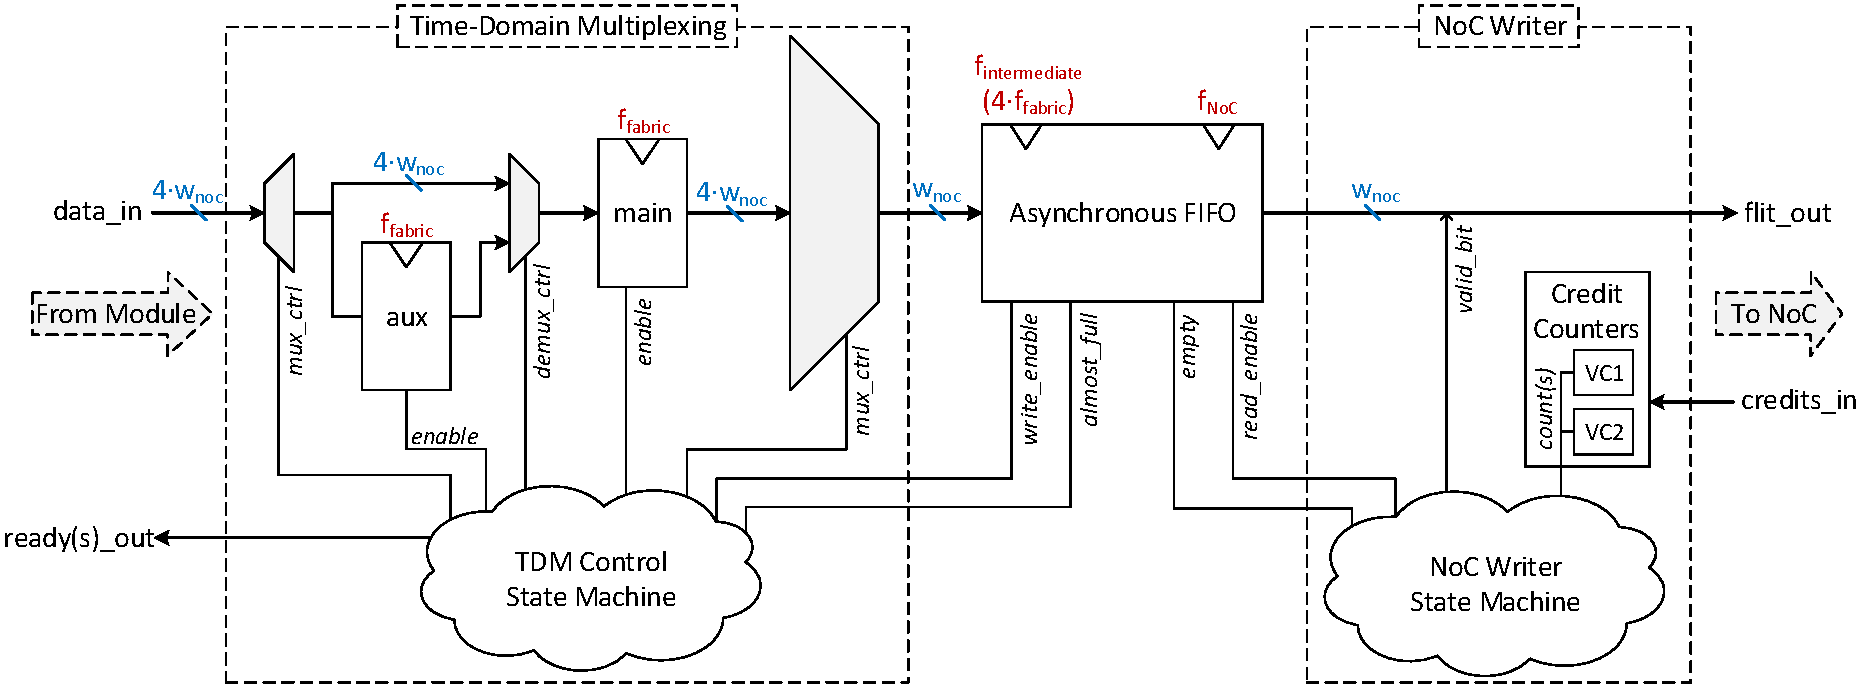
\includegraphics[width=2\columnwidth,keepaspectratio]{images/fpin_detail}
   \label{fpin}
 }
 \\
\subfloat[FabricPort output: from the embedded NoC to the FPGA fabric.]{
   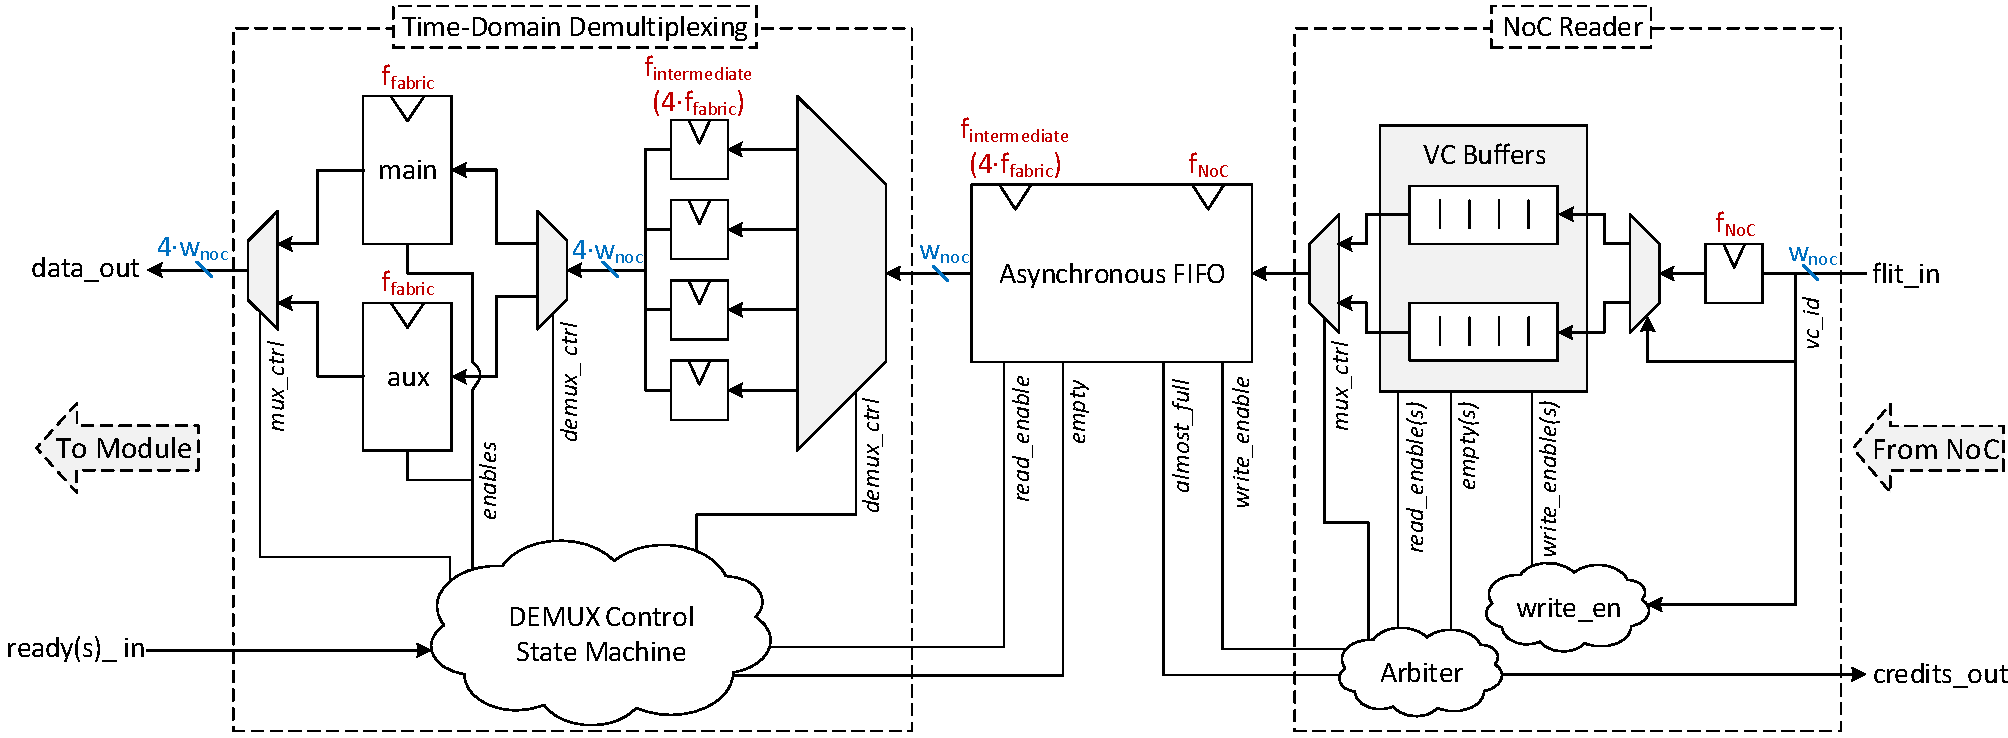
\includegraphics[width=2\columnwidth,keepaspectratio]{images/fpout_detail}
   \label{fpout}
 }
\caption{The FabricPort interfaces the FPGA fabric to an embedded NoC in a flexible way by bridging the different frequencies and widths as well as handling backpressure from both the FPGA fabric and the NoC.}
\label{fabric_port}
\end{figure*}

%----------------------------------------------------------------------------
\subsubsection{FabricPort Input: Fabric$\rightarrow$NoC}
%----------------------------------------------------------------------------

Fig.~\ref{fabric_port} shows a schematic of the FabricPort with important control signals annotated.
The FabricPort input (Fig.~\ref{fpin}) connects the output of a module in the FPGA fabric to an embedded NoC input.
Following the diagram from left to right: data is input to the time-domain multiplexing (TDM) circuitry on each fabric clock cycle and is buffered in the ``main" register.
The ``aux" register is added to provide elasticity. Whenever the output of the TDM must stall there is a clock cycle before the stall signal is processed by the fabric module.
In that cycle, the incoming datum may still be valid, and is therefore buffered in the ``aux" registers.
%To clarify this ready-valid behavior, example waveforms are illustrated in Fig.~\ref{stall_protocol}.
Importantly, this stall protocol ensures that every stall (ready = 0) cycle only stops the input for exactly one cycle ensuring that the FabricPort input does not reduce throughput.

The TDM unit takes four flits input on a slow fabric clock and outputs one flit at a time on a faster clock that is 4\xx as fast as the FPGA fabric -- we call this the intermediate clock.
This intermediate clock is only used in the FabricPort between the TDM unit and the asynchronous FIFO (aFIFO) buffer.
Because it is used only in this very localized region, this clock may be derived locally from the fabric clock by careful design of circuitry that multiplies the frequency of the clock by four.
This is better than generating 16 different clocks globally through phase-locked loops, then building a different clock tree for each router's intermediate clock (a viable but more costly alternative).

The output of the TDM unit is a new flit on each intermediate clock cycle.
Because each flit has a valid bit, only those flits that are valid will actually be written in the aFIFO thus ensuring that no invalid data propagates downstream, unnecessarily consuming power and bandwidth.
The aFIFO bridges the frequency between the intermediate clock and the NoC clock ensuring that the fabric clock can be completely independent from the NoC clock frequency and phase.

The final component in the FabricPort input is the ``NoC Writer".
This unit reads flits from the aFIFO and writes them to the downstream NoC router.
The NoC Writer keeps track of the number of credits in the downstream router to interface to the credit-based backpressure system in the embedded NoC, and only sends flits when there are available credits.
Note that credit-based flow control is by far the most-widely-used backpressure mechanism in NoCs because of its superior performance with limited buffering~\cite{dally_book}.
%Each sender keeps count of the number of credits; the sender has a credit for each available downstream buffer location.
%Therefore, a sender will only send data if it has available credits (telling it that there is buffer space downstream).
%The downstream buffer sends a credit upstream only when it has freed one of its buffer locations by forwarding a flit.

%
%----------------------------------------------------------------------------
\subsubsection{FabricPort Output: NoC$\rightarrow$Fabric}
%----------------------------------------------------------------------------
%

Fig.~\ref{fpout} details a FabricPort output; the connection from an NoC output port to the input of a module on the FPGA fabric.
Following the diagram from right to left: the first component is the ``NoC Reader".
This unit is responsible for reading flits from an NoC router output port and writing to the aFIFO.
Note that separate FIFO queues must be kept for each VC; this is very important as it avoids scrambling data from two packets.
Fig.~\ref{demux} clarifies this point; the upstream router may interleave flits from different packets if they are on different VCs.
By maintaining separate queues in the NoC reader, we can rearrange flits such that flits of the same packet are organized one after the other.

The NoC reader is then responsible for arbitrating between the FIFO queues and forwarding one (entire) packet -- one flit at a time -- from each VC.
We currently implement fair round-robin arbitration and make sure that there are no ``dead" arbitration cycles.
That means that as soon as the NoC reader sees a tail flit of one packet, it has already computed the VC from which it will read next.
The packet then enters the aFIFO where it crosses clock domains between the NoC clock and the intermediate clock.

The final step in the FabricPort output is the time-domain demultiplexing (DEMUX).
This unit reassembles packets (or packet fragments if a packet is longer than 4 flits) by combining 1-4 flits into the wide output port.
In doing so, the DEMUX does not combine flits of different packets and will instead insert invalid zero flits to pad the end of a packet that doesn't have a number of flits divisible by 4 (see Fig.~\ref{demux}).
%This is very much necessary to simplify the output of the NoC into something that is understandable by designers thereby creating an abstracted view of the NoC without complicating design.
This is very much necessary to present a simple interface for designers allowing them to connect design modules to the FabricPort with minimal soft logic.


%
\figvs{1}{demux}{}{``NoC Reader" sorts flits from each VC into a separate queue thereby ensuring that flits of each packet are contiguous. The DEMUX then packs up to four flits together and writes them to the wide output port but never mixes flits of two packets.}
%



%
%---------------------------------------------------------------------------------------------------------
\subsection{IOLinks}
%---------------------------------------------------------------------------------------------------------
%


The FabricPort interfaces between the NoC and the FPGA in a flexible way.
To connect to I/O interfaces, such as external memory interfaces, we can connect through a regular Fabricport interface.
This could be done by simply connecting the I/O interface to soft logic which then connects to a FabricPort as shown in Fig.~\ref{io_fp}.
However, the soft logic between an I/O interface and the FabricPort may be difficult to design for many reasons:

%
\begin{itemize}
    \item Fast I/O interfaces have very stringent timing requirements, making timing closure on any soft logic connecting to it very challenging.
    \item The NoC router may be physically placed far away from the I/O interface, thus heavily-pipelined soft logic is required to connect the two. This may incur significant area and power overhead as the data bandwidth of some I/O interfaces is very large, which translates into a wide data path in the slow FPGA logic. Furthermore, adding pipeline registers would improve timing but typically worsen latency -- a critical parameter of transferring data over some I/Os.
    \item Any solution is specific to a certain FPGA device and will not be portable to another device architecture.
\end{itemize}
%

%
\begin{figure}[t]
\centering
\subfloat[Through the FabricPort.]{
   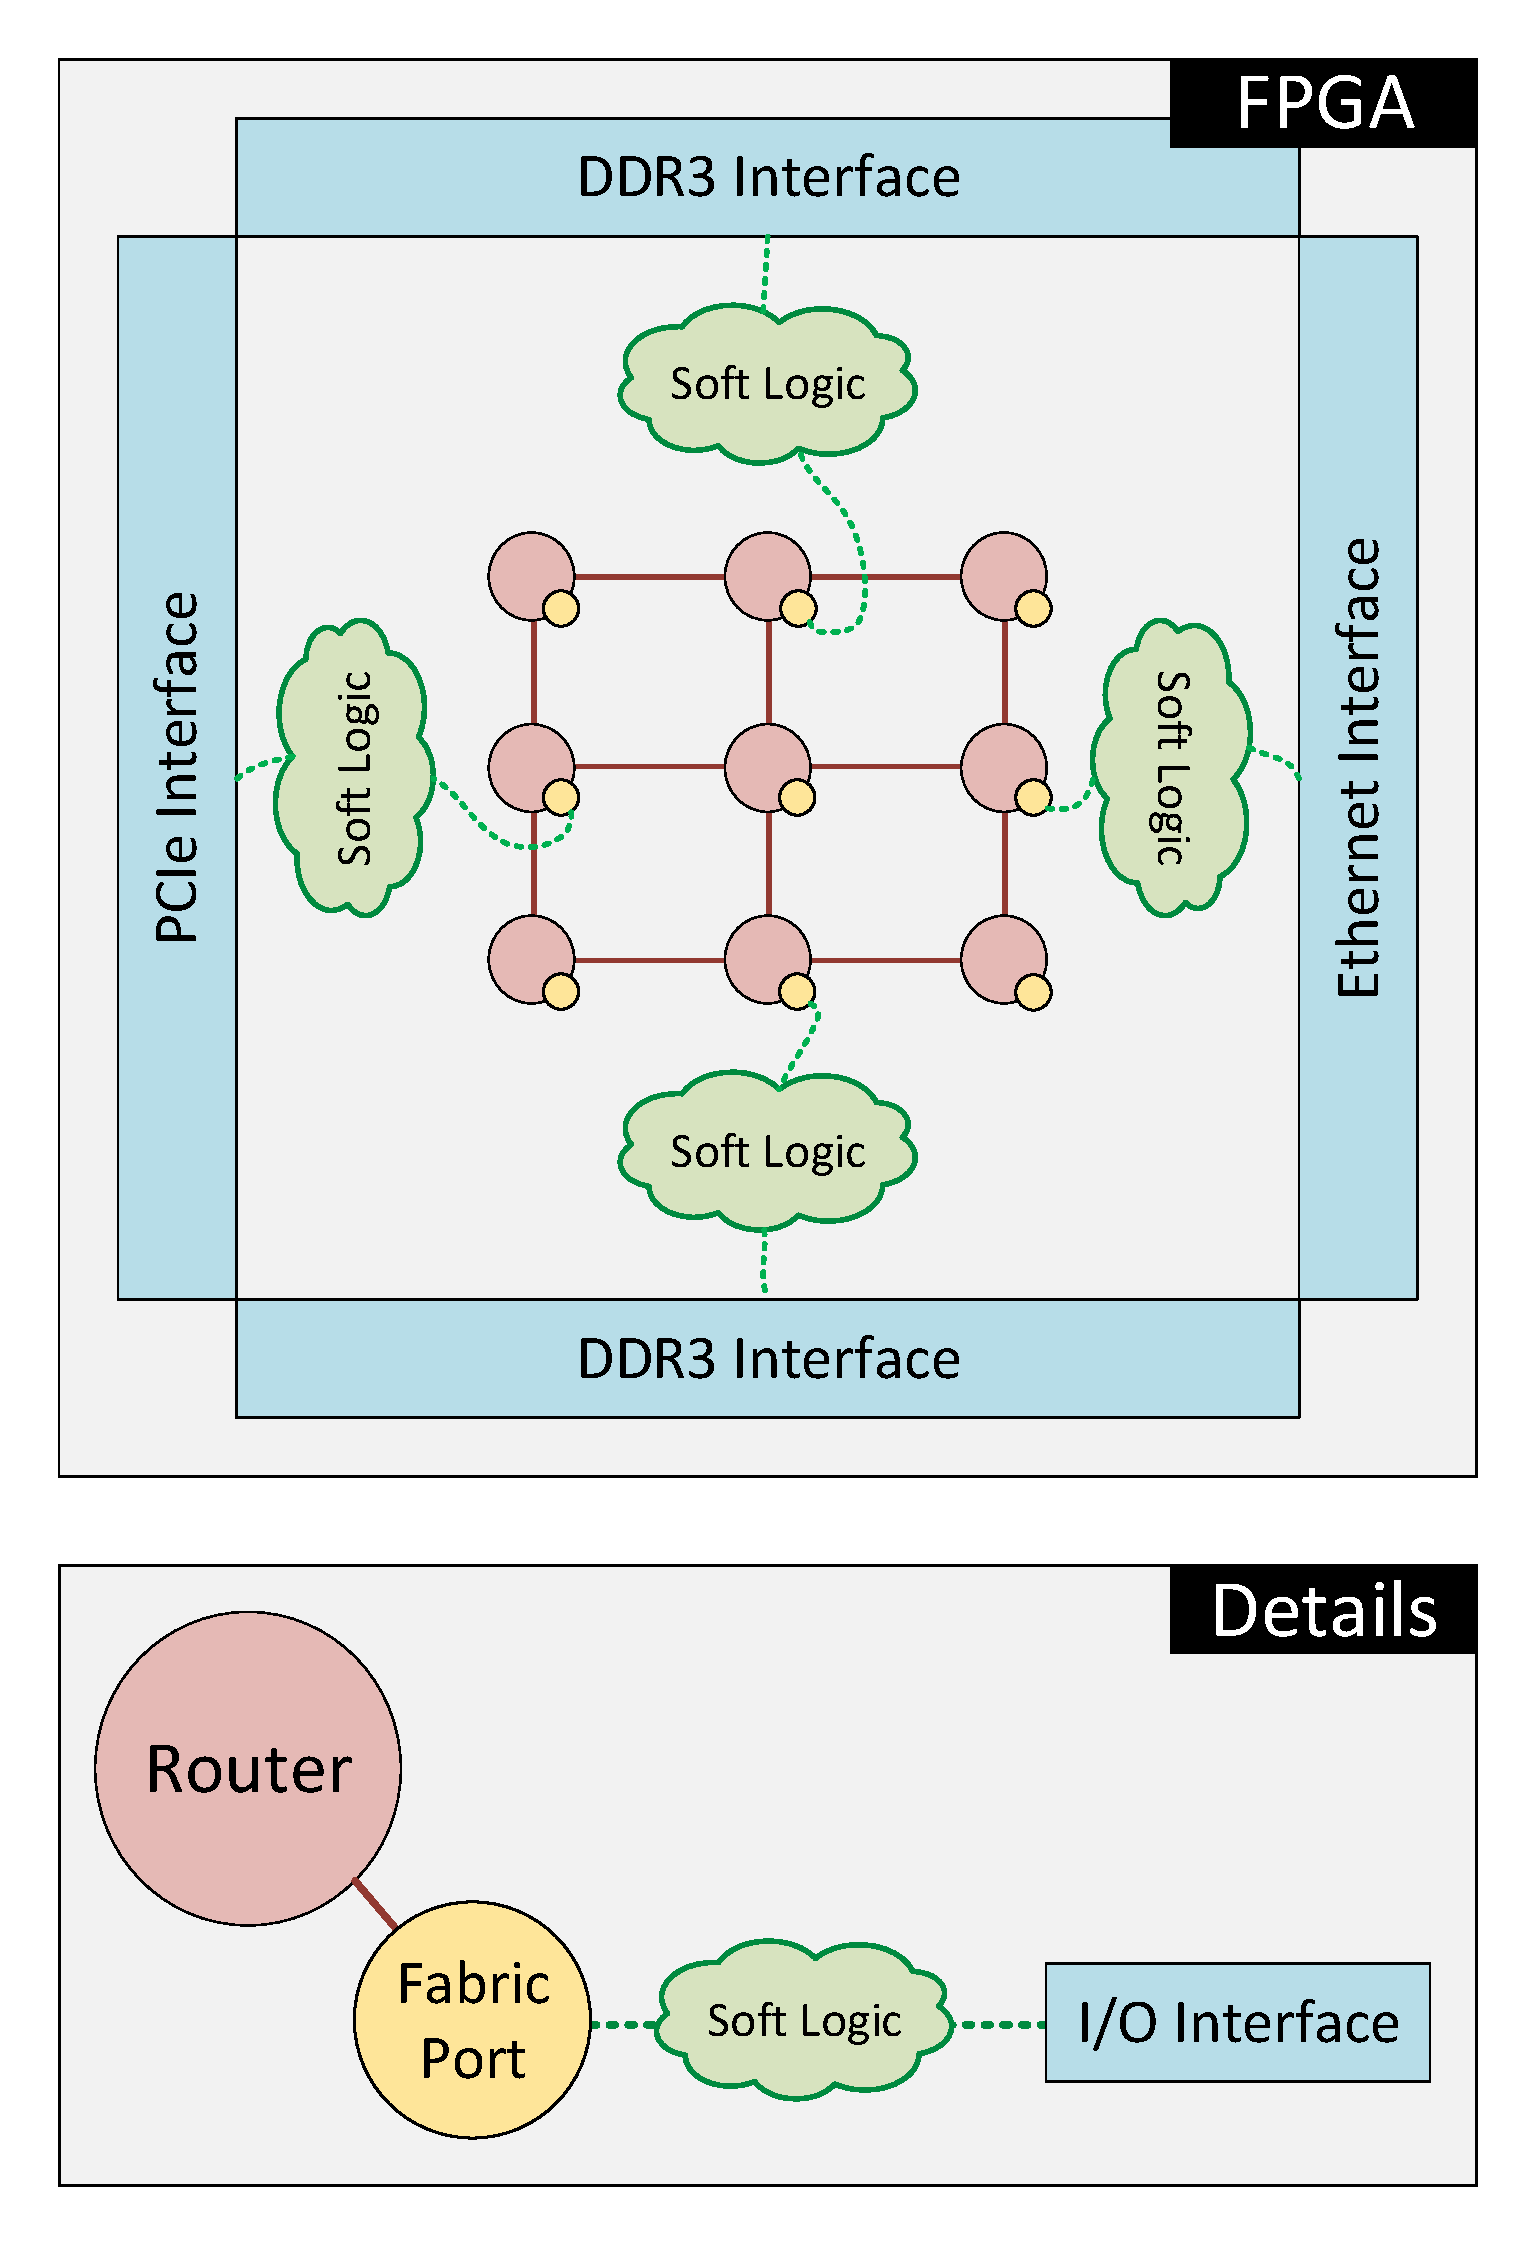
\includegraphics[width=0.49\columnwidth,keepaspectratio, trim = 0cm 0cm 0cm 2.3cm]{images/io_direct}
   \label{io_fp}
 }
\subfloat[Directly using hard IOLinks.]{
   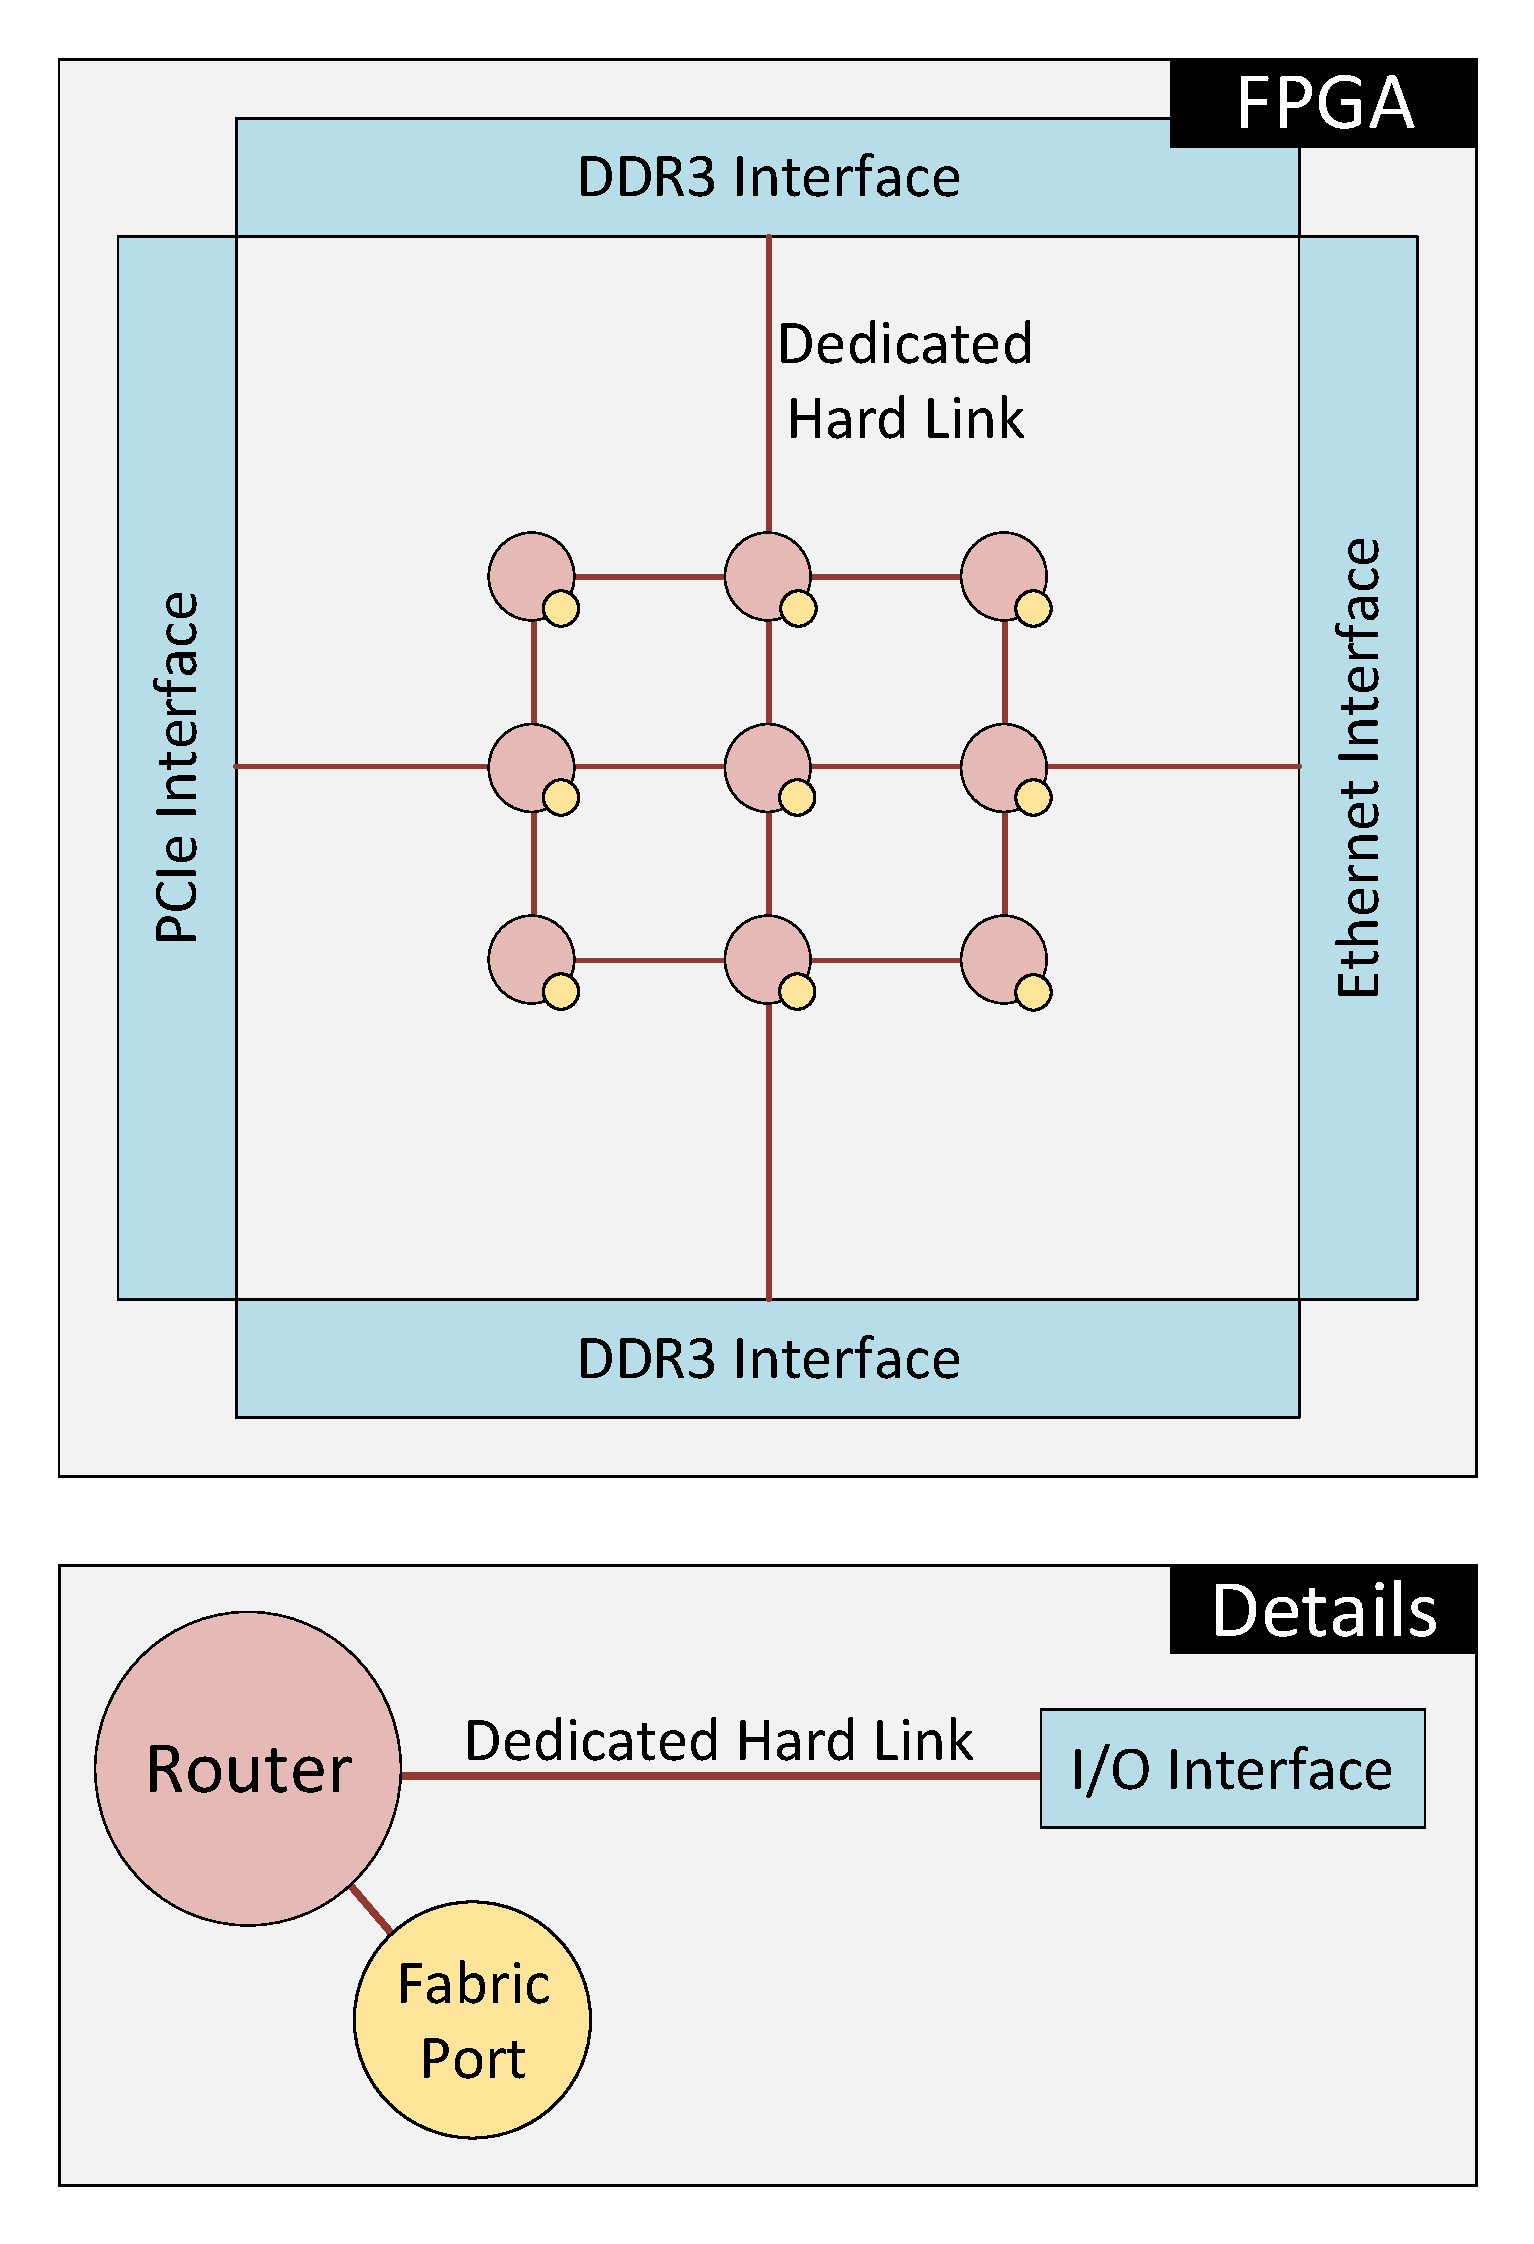
\includegraphics[width=0.49\columnwidth,keepaspectratio, trim = 0cm 0cm 0cm 2.3cm]{images/io_fp}
   \label{io_direct}
 }
\caption{Two options for connecting NoC to I/O interfaces.}
\label{two_options_io}
\end{figure}
%

These shortcomings are the same ones that we use to motivate the use of an embedded NoC instead of a soft bus to distribute I/O data.
Therefore, if we connect to I/O interfaces through the FabricPort, we lose some of the advantages of embedding a system-level NoC.
Instead, we propose connecting NoC routers directly to I/O interfaces using hard links as shown in Fig.~\ref{io_direct}.
In addition, clock-crossing circuitry (such as an aFIFO) will be required to bridge the frequency of the I/O interface and the embedded NoC since they will very likely differ.
We call these direct I/O links with clock crossing ``IOLinks".
They have many advantages:

%
\begin{itemize}
    \item Uses fewer NoC resources since it frees a FabricPort which can be used for something else.
    \item Reduces soft logic utilization conserving area and power.
    \item Reduces data transfer latency between NoC and I/O interfaces because we avoid adding pipelined soft logic.
\end{itemize}
%

One possible shortcoming of IOLinks is the loss of reconfigurability -- it is important to design these I/O links such that they do not rid the FPGA I/O interfaces of any of their built-in flexibility.
IOLinks should be optional by using multiplexers in the I/O interfaces to choose between our IOLinks and the traditional interface to the FPGA logic.
This will maintain the option of directly using I/O interfaces without using IOLinks, thus maintaining the configurability of I/O interfaces.
Note that an IOLink's implementation will be very specific to the I/O interface to which it connects; we study an IOLink to DDR3 interface in Section~\ref{sec_ddr}.

\comment{
To be able to send packets to the directly-connected I/O interfaces, we need to extend NoC addressing to include the directly-connected I/Os.
For example, our proposed NoC has 16 routers and therefore requires 4 addressing bits in its packet format.
However, this NoC can connect up to 16 I/O interfaces along its perimeter (by extending the mesh topology at each side).
We therefore have a maximum of 32 different addresses (16 routers and 16 direct I/Os) for this NoC and we will require 5 address bits instead of 4.
}
%
%

%
%
%
%#############################################################
\section{Design Styles and Constraints with NoC}
\label{sec_fpganoc}
%-0-0-0-0-0-0-0-0-0-0-0-0-0-0-0-0-0-0-0-0-0-0-0-0-0-0-0-0-0-0-
%
%
%
\comment{
\begin{itemize}
	\item in cmps where all data are cache lines and there is a limited number of outstanding requests, and incoming data each has a tag to indicate which it is. processors can resolve exactly what to do with this data.
	\item we want to have streams of data so we can either tag each packet with a order id and add reordering buffers which may be huge and impossible to size, or we can constrain the NoC such that packets always arrive in-order.
	\item this means that we must use deterministic routing algorithms -- we use dor, and we can use VCs but each message class is limited to using only a single VC.
	\item give formal notation for the constraint on VCs -- data originating at a src and going to a dest must stay on the same VC.
	\item an average user should not be aware that the NoC exists: it is simply a portal in which s/he can throw data in and expect it to arrive at the other end.
	\item usually people don't care how efficiently they are actually using their interconnect resources.
	\item advanced designers will want to make best use of the NoC bandwidth/power and can therefore optimize the data size before inserting into the NoC and write custom interfaces in which case they would want to know the min flit width and min packet width -- the former is relevant for latency-insensitive and the latter is relevant for latency-sensitive.
	\item we can use the NoC both in latency-sensitive mode when we establish a permanent channel between two modules (and here we have the advantage of parallel compilation, freedom of placement etc)
	\item or latency-insensitive mode for everything else when we cannot map communication into non-intersecting paths on the NoC.
\end{itemize}
}
%
%

Fig.~\ref{classification} shows the two possibilities of synchronous design styles, as well as two communication protocols that are common in FPGA designs.
%The two design styles are ``latency-insensitive", and ``latency-sensitive". 
In a latency-insensitive system, the design consists of \textit{patient} modules that can be stalled, thus allowing the interconnect between those modules to have arbitrary delay~\cite{Carloni2002}.
Latency-sensitive design, on the other hand, does not tolerate variable latency on its connections, and assumes that its interconnect always has a fixed latency.
In this section we investigate how to map applications that belong to either design style (and any communication protocol) onto the NoC; Fig.~\ref{sys} illustrates this.
We are effectively augmenting the FPGA with a wide stallable network of buffered interconnect that can do flexible switching -- how can we best leverage that new interconnection resource for different design styles? 
And can this embedded NoC be used for both latency insensitive/sensitive design styles, and both communication protocols?

%
\figvs{1}{zl_latency}{trim = 1.7cm 2.4cm 1.7cm 2.0cm, clip}{Zero-load latency of the embedded NoC (including FabricPorts) at different fabric frequencies. Latency is reported as the number of cycles at each frequency. The number of hops varies from 1 hop (minimum) to 7 hops (maximum -- chip diagonal).}
%

%
\figvs{1}{classification}{}{Design styles and communication protocols.}
%

%
\figvs{1}{sys}{}{Mapping latency-sensitive and latency-insensitive systems onto an embedded NoC. We reserve \textit{Permapaths} on the NoC to guarantee a fixed latency and perfect throughput for a latency-sensitive application. For latency-insensitive systems, modules must be encapsulated with wrappers to add stall functionality.}
%


%
%--------------------------------------------------------------------------------------------------------
\subsection{Packet Ordering and Dependencies}
%--------------------------------------------------------------------------------------------------------
%

%
%--------------------------------------------------------------
\subsubsection{Ordering}
%--------------------------------------------------------------
%

Packet-switched NoCs like the one we are using were originally built for chip multiprocessors (CMPs).
CMPs only perform \textbf{memory-mapped} communication; most transfers are cache lines or coherency messages.
Furthermore, processors have built-in mechanisms for reordering received data, and NoCs are typically allowed to reorder packets.
%do not guarantee that packets will arrive in order.

With FPGAs, memory-mapped communication can be one of two main things: (1) Control data from a soft processor that is low-bandwidth and latency-critical -- a poor target for embedded NoCs, or (2) Communication between design modules and on-chip or off-chip memory, or PCIe links -- high bandwidth data suitable for our proposed NoC.
Additionally, FPGAs are very good at implementing \textbf{streaming}, or data-flow applications such as packet switching, video processing, compression and encryption.
These streams of data are also prime targets for using our high-bandwidth embedded NoC.
Crucially, neither memory-mapped nor streaming applications tolerate packet reordering on FPGAs, nor do FPGAs natively support it.
While it may be possible to design reordering logic for simple memory-mapped applications, it becomes \textit{impossible} to build such logic for streaming applications without hurting performance -- we therefore choose to restrict the embedded NoC to perform in-order data transfers only.
Specifically, an NoC is not allowed to reorder packets on a single connection.
%
\begin{defn}
A \textbf{connection} (\textbf{s}, \textbf{d}) exists between a single source (\textbf{s}) and its downstream destination (\textbf{d}) to which it sends data.
\end{defn}
%
\begin{defn}
A \textbf{path} is the sequence of links from \textbf{s} to \textbf{d} that a flit takes in traversing an NoC.
\end{defn}
%

There are two causes of packet reordering.
Firstly, an adaptive route-selection algorithm would always attempt to choose a path of least contention through the NoC; therefore two packets of the same source and destination (same connection) may take different paths and arrive out of order.
Secondly, when sending packets (on the same connection) but different VCs, two packets may get reordered even if they are both taking the same path through the NoC.

To solve the first problem, we only use routing algorithms, in which routes are the same for all packets that belong to a connection.
%
\begin{cond}
\label{routing_constraint}
The same \textbf{path} must be taken by all packets that belong to the same \textbf{connection}.
\end{cond}
%
%
Deterministic routing algorithms such as dimension-ordered routing~\cite{dally_book} fulfill Condition~\ref{routing_constraint} as they always select the same route for packets on the same connection.
%


Eliminating VCs altogether would fix the second ordering problem; however, this is not necessary.
VCs can be used to break message deadlock, merge data streams (Fig.~\ref{merge}), alleviate NoC congestion and may be also used to assign packet priorities thus adding extra configurability to our NoC -- these properties are desirable.
We therefore impose more specific constraints on VCs such that they may still be used on FPGA NoCs.
%
\begin{cond}
All packets belonging to the same \textbf{connection} must use the same VC.
\end{cond}
%


To do this in NoC routers is simple.
Normally, a packet may change VCs at every router hop -- VC selection is done in a VC allocator~\cite{dally_book}.
We replace this VC allocator with a lightweight VC \textit{facilitator} that cannot switch a packet between VCs; instead, it inspects a packet's input VC and stalls that packet until the downstream VC buffer is available.
At the same time, other connections may use other VCs in that router thus taking advantage of multiple VCs.


%
%--------------------------------------------------------------
\subsubsection{Dependencies and Deadlock}
%--------------------------------------------------------------
%

\begin{figure}[t]
\centering
\subfloat[Standard FabricPort output.]{
   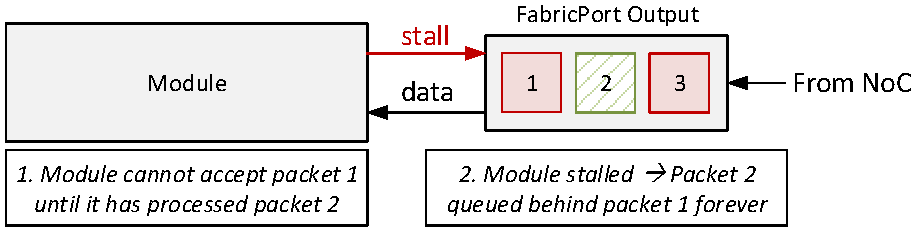
\includegraphics[width=0.9\columnwidth,keepaspectratio]{images/deadlock}
   \label{deadlock}
 }
 \\
\subfloat[Deadlock-free FabricPort output.]{
   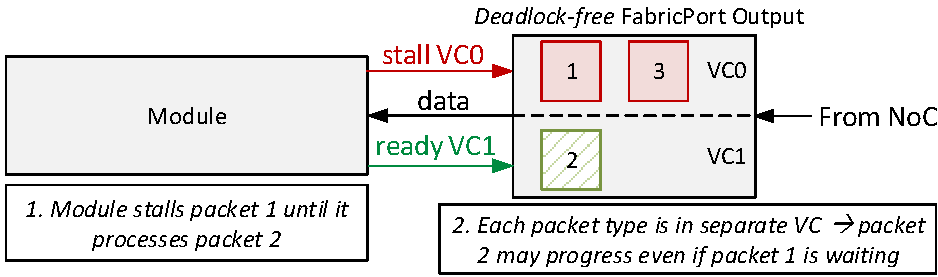
\includegraphics[width=0.9\columnwidth,keepaspectratio]{images/nodeadlock}
   \label{nodeadlock}
 }
\caption{Deadlock can occur if a dependency exists between two message types going to the same port. By using separate VCs for each message type, this deadlock can be broken thus allowing two dependent message types to share a FabricPort output.}
\label{dead}
\end{figure}


Two \textit{message types} may not share a standard FabricPort output (Fig.~\ref{fpout}) if a dependency exists between the two message types.
An example of dependent message types can be seen in video processing IP cores: both control messages (that configure the IP to the correct resolution for example) and data messages (pixels of a video stream) are received on the same port~\cite{altera_vip}.
An IP core may not be able to process the data messages correctly until it receives a control message.

Consider the deadlock scenario in Fig.~\ref{deadlock}.
The module is expecting to receive packet 2 but gets packet 1 instead; therefore it stalls the FabricPort output and packet 2 remains queued behind packet 1 forever.
To avoid this deadlock, we can send each message type in a different VC~\cite{Sorin2011}.
Additionally, we created a deadlock-free FabricPort output that maintains separate paths for each VC -- this means we duplicate the aFIFO and DEMUX units for each VC we have.
There are now two separate ``ready" signals; one for each VC, but there is still only one data bus feeding the module. 
The module can therefore \textit{either} read from VC0 or VC1.
Fig.~\ref{nodeadlock} shows that even if there is a dependency between different messages, they can share a FabricPort output provided each uses a different VC.
%
\begin{cond}
When multiple message types can be sent to a FabricPort, and a dependency exists between the message types, each type must use a different VC.
\end{cond}
%

%
%---------------------------------------------------------------------------------------------------------
\subsection{Latency-Insensitive Design with NoC}
%---------------------------------------------------------------------------------------------------------
%

Latency-insensitive design is a design methodology that decouples design modules from their interconnect by forcing each module to be \textit{patient}; that is, to tolerate variable latency on its inputs~\cite{Carloni2002}.
This is typically done by encapsulating design modules with wrappers that can stall a module until its input data arrives.
This means that a design remains functionally correct, by construction, regardless of the latency of data arriving at each module.
The consequence of this latency tolerance is that a CAD tool can automatically add pipeline stages (called \textit{relay stations}) invisibly to the circuit designer, late in the design compilation and thus improve frequency without extra effort from the designer~\cite{Carloni2002}.

Our embedded NoC is effectively a form of latency-insensitive interconnect; it is heavily pipelined and buffered and supports stalling.
We can therefore leverage such an NoC to interconnect patient modules of a latency-insensitive system as illustrated in Fig.~\ref{sys}. 
Furthermore, we no longer need to add relay stations on connections that are mapped to NoC links, avoiding their overhead.

%
\figvs{0.96}{li_wrappers_overhead}{trim = 1.5cm 3.7cm 1.5cm 3.45cm, clip}{Area and frequency of latency-insensitive wrappers from~\cite{Murray2014} (original), and optimized wrappers that take advantage of NoC buffering (NoC-compatible).}
%

Previous work that investigated the overhead of latency-insensitive design on FPGAs used FIFOs at the inputs of modules in the stall-wrappers to avoid throughput degradation whenever a stall occurs~\cite{Murray2014}.
When the interconnect is an embedded NoC; however, we already have sufficient buffering in the NoC itself (and the FabricPorts) to avoid this throughput degradation, thus allowing us to replace this FIFO -- which is a major portion of the wrapper area -- by a single stage of registers.
We compare the area and frequency of the original latency-insensitive wrappers evaluated in~\cite{Murray2014}, and the NoC-compatible wrappers in Fig.~\ref{li_wrappers_overhead} for wrappers that support one input and one output and a width between 100 bits and 600 bits.
As Fig.~\ref{li_wrappers_overhead} shows, the lightweight NoC-compatible wrappers are 87\% smaller and 47\% faster.

We envision a future latency-insensitive design flow targeting embedded NoCs on FPGAs.
Given a set of modules that make up an application, they would first be encapsulated with wrappers, then mapped onto an NoC such that performance of the system is maximized.


%
%---------------------------------------------------------------------------------------------------------
\subsection{Latency-Sensitive Design with NoC\\(Permapaths)}
%---------------------------------------------------------------------------------------------------------
%

%need to introduce latency insensitive design
Latency-sensitive design requires predictable latency on the connections between modules.
That means that the interconnect is not allowed to insert/remove any cycles between successive data.
Prior NoC literature has largely focused on using circuit-switching to achieve quality-of-service guarantees but could only provide a bound on latency rather than a guarantee of fixed latency~\cite{Goossens2005}.
We analyze the latency and throughput guarantees that can be attained from an NoC, and use those guarantees to determine the conditions under which a latency-sensitive system can be mapped onto a packet-switched embedded NoC.
Effectively, our methodology creates permanent paths with predictable latencies (Permapaths) on our packet-switched embedded NoC.

%
%----------------------------------------------------------------------------
\subsubsection{Latency and Throughput Guarantees}
\label{subsec_guarantees}
%----------------------------------------------------------------------------
%


To ensure that the NoC doesn't stall due to unavailable buffering, we size NoC buffers for maximum throughput, so that we never stall while waiting for backpressure signals within the NoC.
This is well-studied in the literature and is done by sizing our router buffers to cover the \textit{credit round-trip latency}~\cite{dally_book} -- for our system, a buffer depth of 10 suffices.



Fig.~\ref{zl_xput} plots the throughput between any source and destination on our NoC in the absence of contention.
The NoC is running at 1.2~GHz with 1-flit width; therefore, if we send 1 flit each cycle at a frequency lower than 1.2~GHz, our throughput is always perfect -- we'll receive data at the same input rate (one flit per cycle) on the other end of the NoC path. 
In fact, the NoC connection acts as a simple pipelined wire; the number of pipeline stages are equivalent to the zero-load latency of an NoC path; however, it is irrelevant because that latency is only incurred once at the very beginning of data transmission after which data arrives on each fabric clock cycle.
We call this a \textbf{Permapath} through the NoC: a path that is free of contention and has perfect throughput.
As Fig.~\ref{zl_xput} shows, we can create Permapaths of larger widths provided that the input bandwidth of our connection does not exceed the NoC port bandwidth of 22.5~GB/s.
This is why throughput is still perfect with 4~flits$\times$300~MHz for instance.
To create those Permapaths we must therefore ensure two things:
%
\begin{cond}
(Permapaths)
The sending module data bandwidth must be less than or equal to the maximum FabricPort input bandwidth.
\end{cond}
%
\begin{cond}
\label{traf_cond}
(Permapaths)
No other data traffic may overlap the NoC links reserved for a Permapath to avoid congestion delays on those links.
\end{cond}
%
Condition~\ref{traf_cond} be determined statically since our routing algorithm is deterministic; therefore, the mapping of modules onto NoC routers is sufficient to identify which NoC links will be used by each module.


%
\figvs{0.96}{zl_xput}{trim = 1.5cm 3.7cm 1.5cm 3.45cm, clip}{Zero-load throughput of embedded NoC path between any two nodes, normalized to sent data. A throughput of ``1" is the maximum; it means that we receive $i$ flits per cycle, where $i$ is the number of flits we insert in the FabricPort each cycle.}
%

%
%---------------------------------------------------------------------------------------------------------
\subsection{Multicast, Reconvergence and Feedback}
%---------------------------------------------------------------------------------------------------------
%

%
\figvs{0.8}{multicast}{}{Aspects of complex FPGA applications.}
%

A complex FPGA application may include multicast, reconvergence and feedback as shown in Fig.~\ref{multicast} -- we discuss these aspects briefly here but leave the in-depth analysis for future work.
Prior NoC research has shown that packet-switched routers can be augmented with multicast capability at very low area overhead~\cite{Enright2008}.
As for reconvergence, the two branches of a reconvergent path may have different latencies on the embedded NoC with different implications for latency-sensitive and latency-insensitive systems.
A latency-sensitive system may become functionally incorrect in that case; the designer must therefore ensure that the paths are balanced.
For a latency-insensitive system functional correctness is guaranteed but throughput degradation may occur if latencies of the two paths differ by a large amount; prior work has investigated path balancing for latency-insensitive systems~\cite{Lu2003}.
Balancing can be done by selecting two paths of the same length through the NoC (hence same latency) and using registers in the FPGA fabric for fine-grained latency adjustment.
Feedback paths are also tricky to implement on embedded NoCs; this stems from the fact that these connections are typically latency-critical and require very low latency so as not to impede throughput.

While some of these connections can be mapped onto the NoC, not all of them have to be; the embedded NoC is not meant to be an interconnect capable of connecting everything on the FPGA; rather a flexible low-cost (but high bandwidth) interconnect resource that \textit{augments} the current FPGA traditional interconnect. 
Remember that the embedded NoC is 1.3\% of FPGA core area while the FPGA's traditional interconnect accounts for \til50\%~\cite{Lewis2013}.
Traditional interconnect can still be used for latency-critical connections while the embedded NoC can be leveraged for connections on which timing closure is difficult or those that require buffering, stallability, or heavy switching.



%
%

%
%
%#############################################################
%\section{Simulator}
%-0-0-0-0-0-0-0-0-0-0-0-0-0-0-0-0-0-0-0-0-0-0-0-0-0-0-0-0-0-0-
%
%%
%
\comment{
\begin{itemize}
	\item flexible simulator that interfaces modelsim to booksim so we can model any NoC we want on the booksim side and any design we want on modelsim side and still get cycle-accurate results.
	\item interface sends flits and credits
	\item uses systemverilog dpi interface and unix sockets to communicate between the two programs
\end{itemize}
}
%
%

To evaluate the performance of embedded NoCs, we created \texttt{RTL2Booksim}\footnote{\texttt{RTL2Booksim} is available for download at \\\url{www.eecg.utoronto.ca/~mohamed/rtl2booksim.html}}: a simulation framework which allows the co-simulation of hardware description languages (HDL) such as Verilog and VHDL, and a widely-used cycle-accurate NoC simulator called Booksim~\cite{booksim}.


%
%

%
%
%#############################################################
\section{Application Case Studies}
\label{sec_apps}
%-0-0-0-0-0-0-0-0-0-0-0-0-0-0-0-0-0-0-0-0-0-0-0-0-0-0-0-0-0-0-
%
\subsection{Simulator}
\label{sec:sim}
%
%
\comment{
\begin{itemize}
	\item flexible simulator that interfaces modelsim to booksim so we can model any NoC we want on the booksim side and any design we want on modelsim side and still get cycle-accurate results.
	\item interface sends flits and credits
	\item uses systemverilog dpi interface and unix sockets to communicate between the two programs
\end{itemize}
}
%
%

To evaluate the performance of embedded NoCs, we created \texttt{RTL2Booksim}\footnote{\texttt{RTL2Booksim} is available for download at \\\url{www.eecg.utoronto.ca/~mohamed/rtl2booksim.html}}: a simulation framework which allows the co-simulation of hardware description languages (HDL) such as Verilog and VHDL, and a widely-used cycle-accurate NoC simulator called Booksim~\cite{booksim}.


%
%


%
\subsection{DDR3 Memory with IOLink}
\label{sec_ddr}


External memory interfaces, especially to DDRx memory, are some of the most important and highest bandwidth I/O interfaces on FPGAs.
In this section we show how an IOLink can improve both the latency and area-utilization of external memory interfaces.

%
%--------------------------------------
\subsubsection{Memory Interface Components}
%--------------------------------------
%

%
\figvs{0.95}{ddrx_block}{}{Block diagram of a typical DDRx memory interface in a modern FPGA.}
%

Fig.~\ref{ddrx_block} shows a typical FPGA external memory interface.
The PHY is used mainly for clocking, data alignment and calibration of the clock and data delays for reliable operation, and to translate double-rate data from memory to single-rate data on the FPGA.
In modern FPGAs, especially the ones that support fast memory transfers, the PHY is typically embedded in hard logic.
%The PHY presents a \textit{standard} protocol called DFI to the next part of the external memory interface; the memory controller.

The memory controller (see Fig.~\ref{ddrx_block}) is in charge of higher-level memory interfacing.
This includes regularly refreshing external memory; %and computing ECC if that option is enabled.
additionally, addresses are translated into bank, row and column components, which allows the controller to issue the correct memory access command based on the previously accessed memory word.
%Importantly, memory controllers also optimize the order of commands to external memory, to minimize the number of costly accesses.
%An example optimization is the coalescing of memory commands that access the same memory bank or row, thus avoiding costly switches between different memory banks or rows~\cite{xemif}.
The memory controller is sometimes implemented hard and sometimes left soft, but the trend in new devices is to harden the memory controller to provide an out-of-the-box working memory solution~\cite{emif}.
Some designers may want to implement their own high-performance memory controllers to exploit patterns in their memory accesses for instance, therefore, FPGA vendors also allow direct connection to the PHY, bypassing the hard memory controller.
However, hard memory controllers are more efficient and much easier to use making it a more compelling option, especially as FPGAs start being used by software developers (in the context of high-level synthesis and data center computing) who do not have the expert hardware knowledge to design a custom memory controller.

The final component of a memory interface is the multi-ported front end (MPFE).
This component allows access to a single external memory by multiple independent modules.
It consists primarily of FIFO memory buffers to support burst transfers and arbitration logic to select among the commands bidding for memory access.
The MPFE is also sometimes hardened on modern FPGAs.
Beyond the MPFE, a soft bus is required to distribute memory data across the FPGA to any module that requires it.

%
%--------------------------------------
\subsubsection{Rate Conversion}
%--------------------------------------
%

One of the functions of an FPGA memory controller is rate conversion.
This basically down-converts the data frequency from the high memory frequency (\til1~GHz) to a lower FPGA-compatible frequency (\til200~MHz).
All modern memory controllers in FPGAs operate at quarter rate; meaning, the memory frequency is down-converted 4\xx and memory width is parallelized eightfold\footnote{Width is multiplied by 8 during quarter-rate conversion because DDRx memory data operates at double rate (both positive and negative clock edges) while the FPGA logic is synchronous to either a rising or falling clock edge}.
Modern FPGA DDR4 memory speeds go up to 1333~MHz (in Xilinx Ultrascale+ for example~\cite{xemif}); at quarter rate, this translates to 333~MHz in the FPGA fabric which is challenging to achieve.
Quarter-rate conversion is \textit{necessary} to be able to use fast DDRx memory on current FPGAs -- how else can we transport and process fast memory data at the modest FPGA speed?
However, there are both performance and efficiency disadvantages that arise due to quarter-rate conversion in the memory controller.

\textbf{Area Overhead:} Down-converting frequency means up-converting data width from 128-bits (at single data rate) to 512-bits.
This 4\xx difference increases the area utilization of the memory controller, the MPFE (including its FIFOs), and any soft bus that distributes memory data on the FPGA.

\textbf{Latency Overhead:} Operating at the lower frequency increases memory transfer latency.
This is mainly because each quarter-rate clock cycle is much slower (4\xx slower) than a full-rate equivalent.

%
%--------------------------------------
\subsubsection{Proposed IOLink}
%--------------------------------------
%

We propose directly connecting an NoC link to I/O interfaces.
For the external memory interface, we propose connecting an IOLink to the AXI port after the hard memory controller (see Fig.~\ref{ddrx_block}).
We also propose implementing a memory controller that supports full-rate memory operations, even at the highest memory speeds.
This topology leverages the high speed and efficiency of a full-rate controller, and avoids the costly construction of a MPFE and soft bus to transport the data.
Instead, an efficient embedded NoC fulfills the function of both the MPFE and soft bus in buffering and transporting DDRx commands and data, furthermore, it does so at full-rate memory speed and lower latency.

Table~\ref{lat_comp_emif} details the latency breakdown of a memory read transaction when fulfilled by a current typical memory interface, and an estimate of latency when an embedded NoC is connected directly to a full-rate memory controller.
We use the latency of the memory chip, PHY and controller from Altera's datasheets~\cite{emif}.
For the MPFE, we estimate that it will take at least 2 system clock cycles\footnote{We define a ``system clock cycle" to be equivalent to the quarter-rate speed of the memory controller in our examples.} (equivalent to 8 memory clock cycles) to buffer data in a burst adapter and read it back out -- this is a very conservative estimate on the latency of a hard MPFE.
To evaluate the soft bus, we generate buses in Altera's Qsys system integration tool with different levels of pipelining.
Only highly pipelined buses (3-5 stages of pipelining) can achieve timing closure for a sample 800~MHz memory speed (200~MHz at quarter rate)~\cite{micro}.
The round-trip latency of these buses in the absence of any traffic is 6-11 system clock cycles (depending on the level of pipelining).

To estimate the embedded NoC latency in Table~\ref{lat_comp_emif}, we used the zero-load latency from Fig.~\ref{zl_latency}.
The round-trip latency consists of the input FabricPort latency, the output FabricPort latency and twice the link traversal latency.
At a 300~MHz fabric (system) frequency, FabricPort input latency is \til2 cycles, FabricPort output latency is 3 cycles and link traversal latency ranges between 1.5-6 cycles depending on the number of routers traversed.
This adds up to a round-trip latency between 8-17 system clock cycles.

%

\renewcommand{\arraystretch}{1.25}
\begin{table}[!t]
\centering
    \caption{Read transaction latency comparison between a typical FPGA quarter-rate memory controller, and a full-rate memory controller connected directly to an embedded NoC link. Latency is measured in full-rate memory clock cycles.}
    \label{lat_comp_emif}
\begin{tabular}{lc|lc}
    \toprule
    \multicolumn{2}{c|}{Current System}&\multicolumn{2}{|c}{NoC-Enhanced System}\\
    \toprule
    Component                 & Latency & Component              & Latency \\
    \midrule
	Memory                    & 5-11     & Memory                 & 5-11    \\
    PHY ($\frac{1}{4}$-rate)        & 22-28    & PHY (full-rate)        & 4       \\
	Controller ($\frac{1}{4}$-rate) & 28       & Controller (full-rate) & 15      \\
    \hline
    MPFE                      &  $>$8    & MPFE                   &   --     \\
    \hline
    Soft Bus                  &  24-44   & Hard NoC               & 32-68    \\
    \hline
    Total                     & 87-119   & Total                  & 56-98   \\
    \hline
    \multicolumn{4}{c}{Speedup = 1.2--1.6\xx}\\
    \bottomrule
\end{tabular}
\end{table}
\renewcommand{\arraystretch}{1}
%

As Table~\ref{lat_comp_emif} shows, the embedded NoC can improve latency by approximately 1.2--1.6\xx.
Even though the embedded NoC has a higher round-trip latency compared to soft buses, latency improves because we use a full-rate memory controller, and avoid a MPFE.
We directly transport the fast memory data using an NoC link, and only down-convert the data at a FabricPort output at the destination router where the memory data will be consumed.
This undoubtedly reduces area utilization as well.
More importantly, an embedded NoC avoids time-consuming timing closure iterations when connecting to an external memory interface, and improves area and power as shown in prior work~\cite{micro}.
%In prior work, we quantified the efficiency and productivity gains of using an embedded NoC compared to a soft bus in connecting to external memory interfaces~\cite{micro}.

%
%

%
\subsection{JPEG Compression}
%
%
\comment{
\begin{itemize}
	\item look at jpeg compression for instance -- conforms to our constraints for a design that can map latency-sensitively onto the NoC
	\item establish communication channels and data arrives each cycle -- we don't even need the ready signals
	\item what advantages does this bring? lets try placing the modules connecting to the routers or connecting together
	\item how much global interconnect does it save?
	\item present a simple cad algo to say whether this app can be mapped latency-sensitvely or not? and give candidate solutions if possible
\end{itemize}
}
%---------------------------------------------------------------------------------------------------------------------------------------------------

%
\figvs{1}{jpeg_app}{}{Single-stream JPEG block diagram.}
%

We use a streaming JPEG compression design from~\cite{jpeg_opencore}.
The application consists of three modules as shown in Fig.~\ref{jpeg_app}; discrete cosine transform (DCT), quantizer (QNR) and run-length encoding (RLE).
The single pipeline shown in Fig.~\ref{jpeg_app} can accept one pixel per cycle and a data strobe that indicates the start of 64 consecutive pixels forming one (8$\times$8) block on which the algorithm operates~\cite{jpeg_opencore}.
The components of this system are therefore latency-sensitive as they rely on pixels arriving every cycle, and the modules do not respond to backpressure.

We parallelize this application by instantiating multiple (10--40) JPEG pipelines in parallel; which means that the connection width between the DCT, QNR and RLE modules varies between 130~bits and 520~bits.
Parallel JPEG compression is an important data-center application as multiple images are often required to be compressed at multiple resolutions before being stored in data-center disk drives; the back-end of large social networking websites and search engines.
We implemented this parallel JPEG application using direct point-to-point links, then mapped the same design to use the embedded NoC between the modules using \textbf{Permapaths} similarly to Fig.~\ref{sys}.
Using the \texttt{RTL2Booksim} simulator, we connected the JPEG design modules through the FabricPorts to the embedded NoC and verified functional correctness of the NoC-based JPEG.
Additionally, we verified that throughput (in number of cycles) was the same for both the original and NoC versions; however, there are \til8 wasted cycles (equivalent to the zero-load latency of three hops) at the very beginning in the NoC version while the NoC link pipeline is getting populated with valid output data -- these 8 cycles are of no consequence.

%---------------------------------------------------------------------------------------
\subsubsection{Frequency}
%---------------------------------------------------------------------------------------

To model the physical design repercussions (placement, routing, critical path delay) of using an embedded NoC, we emulated embedded NoC routers on FPGAs by creating 16 design partitions in Quartus~II that are of size 7$\times$5$=$35 logic clusters -- each one of those partitions represents an embedded hard NoC router with its FabricPorts and interface to FPGA (see Fig.~\ref{heat_map} for chip plan).
We then connected the JPEG design modules to this emulated NoC.
Additionally, we varied the physical location of the QNR and RLE modules (through location constraints) from ``close" together on the FPGA chip to ``far" on opposite ends of the chip.
Note that the DCT module wasn't placed in a partition as it was a very large module and used most of the FPGA's DSP blocks.

%
\figvs{1}{jpeg_freq}{trim = 1.5cm 3.7cm 1.5cm 3.45cm, clip}{Frequency of the parallel JPEG compression application with and without an NoC. The plot ``with NoC" is averaged for the two cases when it's ``close" and ``far" with the standard deviation plotted as error bars. Results are averaged over 3 seeds.}
%

Using location constraints, we investigated the result of a stretched critical path in an FPGA application.
This could occur if the FPGA is highly utilized and it is difficult for the CAD tools to optimize the critical path as its endpoints are forced to be placed far apart, or when application modules connect to I/O interfaces and are therefore physically constrained far from one another.
Fig.~\ref{jpeg_freq} plots the frequency of the original parallel JPEG and the NoC version.
In the ``close" configuration, the  frequency of the original JPEG is higher than that of the NoC version by \til5\%. 
This is because the JPEG pipeline is well-suited to the FPGA's traditional row/column interconnect.
With the NoC version, the wide point-to-point links must be connected to the smaller area of 7$\times$5 logic clusters (area of an embedded router); making the placement less regular and on average slightly lengthening the critical path.

%
\figvs{1}{jpeg_pipes}{trim = 1.5cm 3.3cm 1.5cm 3.77cm, clip}{Frequency of parallel JPEG with 40 streams when we add 1-4 pipeline stages on the critical path. Frequency of the same application when connected to the NoC is plotted for comparison. Results are averaged over 3 seeds.}
%

The advantage of the NoC is highlighted in the ``far" configuration when the QNR and RLE modules are placed far apart thus stretching the critical path across the chip diagonal.
In the NoC version, we connect to the closest NoC router as shown in Fig.~\ref{heat_map} -- on average, the frequency improved by \til80\%.
Whether in the ``far" or ``close" setups, the NoC-version's frequency only varies by \til6\% as the error bars show in Fig.~\ref{jpeg_freq}.
By relying on the NoC's predictable frequency in connecting modules together, the effects of the FPGA's utilization level and the modules' physical placement constraints become localized to each module instead of being a global effect over the entire design.
Modules connected through the NoC become timing-independent making for an easier CAD problem and allowing parallel compilation.


With additional design effort, a designer of the original (without NoC) system would identify the critical path and attempt to pipeline it so as to improve the design's frequency.
This design$\rightarrow$compile$\rightarrow$repipeline cycle hurts designer productivity as it can be unpredictable and compilation could take days for a large design~\cite{Murray2014}.
We plot the frequency of our original JPEG with 40 streams in the ``far" configuration after adding 1, 2, 3, and 4 pipeline registers on the critical path, both with and without register retiming optimizations, and we compare to the NoC version frequency in Fig.~\ref{jpeg_pipes}.
The plot shows that the frequency of the pipelined version never becomes as good as that of the NoC version even with 4 pipeline stages -- the NoC version is 10\% better than original JPEG with pipelining.

\comment{
The plot shows two things.
First, the frequency of the pipelined version never becomes as good as that of the NoC version even with 4 pipeline stages on the critical path -- on average, there is a 10\% difference in frequency.
Secondly, It doesn't really matter how many pipeline registers we place on the critical path, nor does it matter much whether register retiming is enabled. 
This is because register retiming occurs before placement and routing in the CAD flow, and therefore has no physical awareness on where the register will actually be placed on the FPGA device.
}


%---------------------------------------------------------------------------------------
\subsubsection{Interconnect Utilization}
%---------------------------------------------------------------------------------------

%
\begin{table}[!t]
\centering
\begin{small}
    \caption{Interconnect utilization for JPEG with 40 streams in ``far" configuration. Relative difference between NoC version and the original version is reported.}
    \label{wire_util}
    \begin{tabular}{cccc}
    \toprule
    \multicolumn{2}{c}{Interconnect Resource}       & Difference & Geomean \\
    \midrule
	\multirow{2}{*}{Short}   & Vertical (C4)         & +13.2\%   & \multirow{2}{*}{+10.2\%} \\
	                         & Horizontal (R3,R6)   & +7.8\% & \\
	\midrule
	\multirow{2}{*}{Long} & Vertical (C14)           & -47.2\% & \multirow{2}{*}{-38.6\%}\\
	& Horizontal (R24)                              & -31.6\%  & \\
    \bottomrule
	\end{tabular}
    \begin{tabular}{cccc}
	\multicolumn{4}{c}{Wire naming convention: C=column, R=row, }\\
	\multicolumn{4}{c}{followed by number of logic clusters of wire length.}\\
    \end{tabular}
\end{small}
\end{table}
%

Table~\ref{wire_util} quantifies the FPGA interconnect utilization difference for the two versions of 40-stream ``far" JPEG.
The NoC version reduces long wire utilization by \til40\% but increases short wire utilization by \til10\%.
Note that long wires are scarce on FPGAs, for the Stratix~V device we use, there are 25\xx more short wires than there are long wires.
By offloading long connections onto an NoC, we conserve much of the valuable long wires.

%
\figvs{1}{heat_map}{}{Heat map showing total wire utilization for the NoC version, and only long-wire utilization for the original version of the JPEG application with 40 streams when modules are spaced out in the ``far" configuration. In hot spots, utilization of scarce long wires in the original version goes up to 100\%, while total wire utilization never exceeds 40\% for the NoC version.}
%

Fig.~\ref{heat_map} shows wire utilization for the two versions of 40-stream ``far" JPEG and highlights that using the NoC does not produce any routing hot spots around the embedded routers.
As the heat map shows, FPGA interconnect utilization does not exceed 40\% in that case.
Conversely, the original version utilizes long wires heavily on the long connection between QNR$\rightarrow$RLE, with utilization going up to 100\% in hot spots at the terminals of the long connection as shown in Fig.~\ref{heat_map}.


%
%
%
\subsection{Ethernet Switch}
%
%
%\begin{itemize}
%	\item performance of a packet-switching fabric using the NoC -- different topologies, includes interface
%\end{itemize}
%
%

%\subsubsection{Design}

%Packet switching applications switch data that has been separated into packets.
%These packets include control information that describe various attributes of the payload, such as its source and destination.
%Unlike other data streaming applications, the distribution of packet sources and destinations can vary widely, and are rarely known before runtime.
%A Ethernet switch must be capable of completing packet transmission under any possible traffic condition.

\begin{figure*}[t] \centering \vspace{0cm}
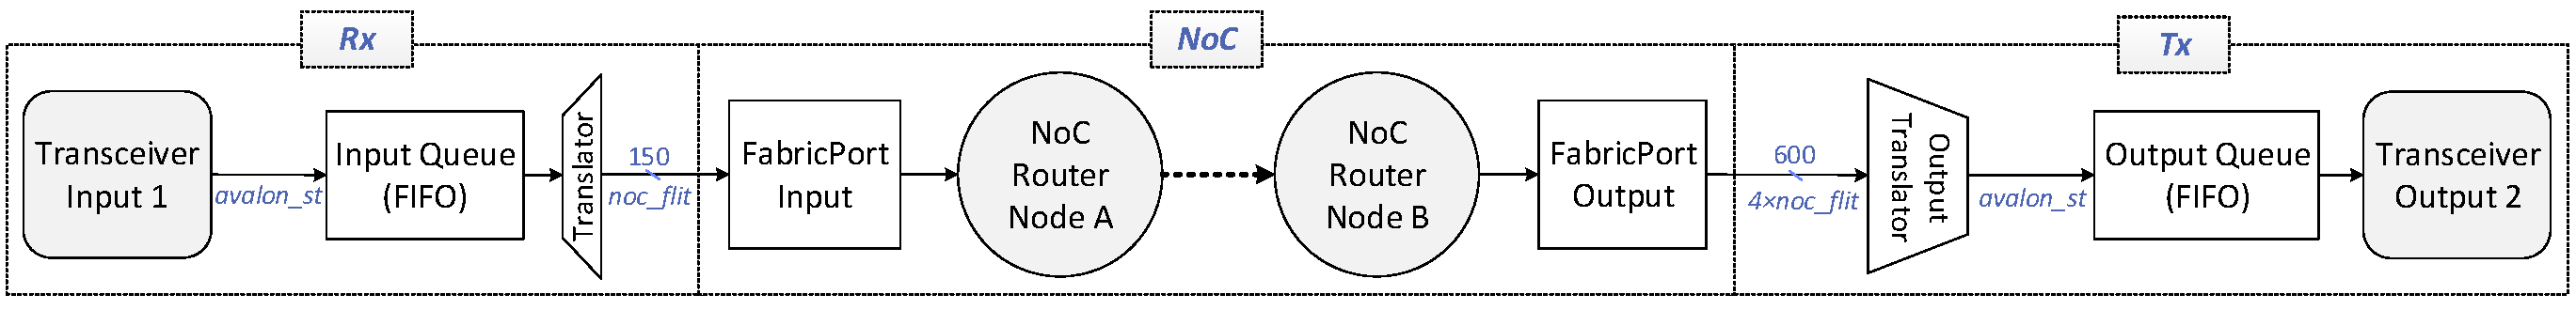
\includegraphics[width=0.95\textwidth, trim = 0cm 0.15cm 0cm 0.3cm]{images/complete-switch-path-new.pdf}
\caption{Functional block diagram of one path through our NoC Ethernet switch.}
\label{fig:switch-blk-diagram}
\vspace{0cm}
\end{figure*}


%
%\figvs{0.9}{ethernet}{}{Block diagram of NoC-based Ethernet switch.}
%

One of the most important and prevalent building blocks of communication networks is the Ethernet switch.
The embedded NoC provides a natural back-bone for an Ethernet switch design, as it includes (1) switching and (2) buffering within the NoC routers, and (3) a built-in backpressure mechanism for flow control.
Recent work has revealed that an Ethernet switch achieves significant area and performance improvements when it leverages an NoC-enhanced FPGA~\cite{Bitar2014}.
We describe here how such an Ethernet switch can take full advantage of the embedded NoC, while demonstrating that it considerably outperforms the best previously proposed FPGA switch fabric design~\cite{dai-zhu}.

%The NoC provides two possible design options for transporting packetized data, as listed below.
%We will refer to the streaming data packets as ``stream packets'' in order to avoid confusion with the NoC's packets.
%
%\begin{enumerate}
%
%\item \textbf{Encapsulate} each stream packet into multiple NoC packets.
%A NoC packet holds one data beat from the stream packet, including both payload and all control information.
%The stream packet's control data does not need to be read.
%
%\item \textbf{Translate} each stream packet into a single NoC packet.
%The stream packet's start-of-packet (SOP) and end-of-packet (EOP) data beats are sent in the head and tail flits of the NoC packet, respectively.
%Thus, the SOP and EOP signals are stripped from the stream packet before being sent through the NoC.
%
%\end{enumerate}
%
%Encapsulating the data is the simplest design option, as it only requires logic to read the data's destination before sending it through the NoC.
%Additionally, since it breaks up stream packets into smaller, fixed-size NoC packets, it can potentially achieve better latency.
%However, this design method comes with several limitations.
%Breaking packets up into smaller units introduces the possibility of packet re-ordering and packet interleaving in the NoC.
%%A centralized scheduler, similar to ones used in other Ethernet switch designs, would be needed to prevent this from occurring.
%To remedy this, each NoC packet would need additional control data indicating the flit ID and source, as well as complex re-ordering logic at the output.
%On the other hand, translating each stream packet to a NoC packet prevents packet re-ordering/interleaving, thus removing this complexity.
%Although translation requires some additional logic to perform the conversion from stream packet to NoC packet, and vice versa, this logic is far simpler than the re-ordering logic necessary for encapsulation.
%Thus, we recommend that Ethernet switch designs translate, rather than encapsulate, stream packets into NoC packets.
%%By building and simulating this design, we show that it better leverages the NoC for packet-switching applications.

%\begin{figure}[t] \centering \vspace{0cm}
%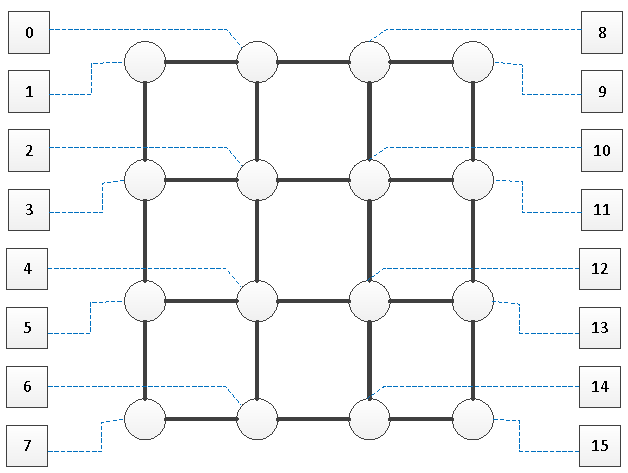
\includegraphics[width=0.4\textwidth]{images/16-node-mesh.pdf}
%\caption{Each of the 16 transceiver nodes (squares) connect to a unique NoC router (circles) through the FPGA's fabric (dashed lines)}
%\label{fig:16mesh}
%\vspace{0cm}
%\end{figure}

%Our design consists of a 16$\times$16 10-Gigabit Ethernet switch.
The embedded NoC is used in place of the switch's crossbar.
For a 16$\times$16 switch, each of the 16 transceiver nodes are connected to one of the 16 NoC routers via the FPGA's soft fabric.
%To transport 10~Gb/s data, the soft fabric is set to run at 156.25 MHz for 64-bit wide data.
%Each transceiver-to-router path consists of buffering and logic to convert stream packets to NoC packets, and vice-versa.
%The transceiver-to-router paths complete the flow shown in Fig.~\ref{fig:switch-blk-diagram}.
Fig.~\ref{fig:switch-blk-diagram} shows the path between transceiver 1 and transceiver 2; in our 16$\times$16 switch there are 256 such paths from each input to each output.
%On the receive path (\textit{Rx}), two stream flits (\textit{avalon\textunderscore st}) are joined together (\textit{2$\times$avalon\textunderscore st}) before being inserted into an input queue.
On the receive path (\textit{Rx}), Ethernet data is packed into NoC flits before being brought to the FabricPort input.
The translator sets NoC control bits such that one NoC packet corresponds to one Ethernet frame.
For example, a 512-byte Ethernet frame is converted into 32 NoC flits.
%If the NoC router's input fabric port is ready to accept data, the input queue ejects flits to the translator, which adds the necessary NoC control bits and strips the unnecessary Avalon Stream control bits (valid, SOP, EOP) before injecting the newly-created NoC flit into the fabric port.
After the NoC receives the flit from the FabricPort, it steers the flit to its destination, using dimension-order XY routing.
%\footnote{The impact of routing algorithms on NoC-based Ethernet switch performance was investigated by Bitar \textit{et al.}~\cite{Bitar2014}.}
%On the transmit path (\textit{Tx}), round-robin arbitration logic is needed, as the FabricPort can output up to four NoC flits from the same packet in the same cycle (see Section~\ref{sec_fabricport}).
%On the transmit path (\textit{Tx}), the translator uses demultiplexing in order to convert the FabricPort output width (600~bits) to the output queue width (150~bits).
On the transmit path (\textit{Tx}), the NoC can output up to four flits (600~bits) from a packet in a single system clock cycle -- this is demultiplexed in the output translator to the output queue width (150~bits).
This demultiplexing accounts for most of the translators' area in Table~\ref{tbl:hcost}.
The translator also strips away the NoC control bits before inserting the Ethernet data into the output queue.
%The output queue waits for an end-of-packet signal before beginning transmission.
%Although we set the queue size to be 64 bits wide and 512 words deep, this can be varied depending on the needs of the switch's particular application.

We synthesized the soft logic on a Stratix~V device, and
The design is synthesized on a Stratix V device and show the resource utilization in Table~\ref{tbl:hcost}.
Because we take advantage of the NoC's switching and buffering our switch is \til3$\times$ more area efficient than previous FPGA Ethernet switches~\cite{dai-zhu} even when accounting for the complete embedded NoC area.

%The buffering mechanism used by our switch is considered combined input/output queued (CIOQ).
%However, our Ethernet switch has important differences from previously proposed CIOQ architectures~\cite{minkenberg2000combined}.
%The NoC already provides built-in flow control for handling data being sent from multiple sources to a single destination.
%Thus, no centralized scheduling logic or additional flow control signals between the inputs and outputs are necessary, resulting in significant complexity savings.
%%This would not have been possible if the design had encapsulated rather than translated the data, as centralized scheduling logic would have been necessary to
%Additionally, the NoC mitigates head-of-line blocking (HOL) by buffering packets within the NoC rather than within the input queues.
%Typically, CIOQ architectures use virtual output queues (VOQ) to mitigate HOL~\cite{minkenberg2000combined}, thus revealing additional hardware cost savings for our NoC-based Ethernet switch design.

% --> Only talk about the replacement of scheduling logic by NoC backpressuring. Leave HoL discussion to journal paper?

%\begin{itemize}
%
%\item \textbf{No scheduling logic.} In nearly all Ethernet switch designs, scheduling logic is necessary to control which inputs are granted access to the switch crossbar.
%
%\item \textbf{No head-of-line blocking (HOL).}
%
%\end{itemize}

% introduce concept of translating data packets to NoC packets along with both options
% describe design (with block diagram) for 16x16 10~Gb/s
% illustrate inherent benefits of this switch: no centralized scheduler needed, no VOQs needed for HOL

%\subsubsection{Evaluation}

Two important performance metrics for Ethernet switch design are bandwidth and latency~\cite{elhanany2005network}.
The bandwidth of our NoC-based Ethernet switch is limited by the supported bandwidth of the embedded NoC.
As described in Section~\ref{sec:hnoc}, the NoC's links have a bandwidth capacity of 22.5 GB/s (180~Gb/s).
Since some of this bandwidth is used to transport packet control information, the NoC's links can support up to 153.6~Gb/s of Ethernet data.
%The worst case traffic pattern that the NoC-crossbar must support is the pattern that places the highest demand on a NoC link while driving the NoC's sinks at no higher than the line rate, $R$ ($R = 10$~Gb/s in our design).
%Analysis of the 16-node mesh reveals that the maximum NoC channel load is $3R$.
%Thus, the maximum supported bandwidth per node for our Ethernet switch is $R = 51.2$~Gb/s, or an aggregate bandwidth of 819.2~Gb/s.
Analysis of the worst case traffic in a 16-node mesh shows that the NoC can support a line rate of one third its link capacity, i.e. 51.2~Gb/s~\cite{Bitar2014}.
While previous work on FPGA switch design has achieved up to 160~Gb/s of aggregate bandwidth~\cite{dai-zhu}, our switch design can achieve 51.2$\times$16 = 819.2~Gb/s by leveraging the embedded NoC.
We have therefore implemented a programmable Ethernet switch with 16 inputs/outputs that is capable of either 10~Gb/s, 25~Gb/s or 40~Gb/s -- three widely used Ethernet standards.

%
%
\begin{table}[!t]
\centering
\begin{small}
    \caption{Hardware cost breakdown of an NoC-based 10-Gb Ethernet switch on a Stratix V device.}
    \label{tbl:hcost}
    \begin{tabular}{ccccccc}
    \toprule
     & 10GbE & I/O & Translators & \textbf{Total} \\
     & MACs & Queues &  & & \\
    \midrule
	ALMs & 24000  & 3707 &  3504 & \textbf{31211} \\
	%ALUTs & 32016 & 5616 & 2352 & \textbf{41648} \\
	%Regs  & 49232 & 3264 & 17840 & \textbf{53696} \\
	M20Ks & 0    & 192   & 0 & \textbf{192}   \\
    \bottomrule
    \end{tabular}
\end{small}
\end{table}
%
%

\begin{figure}[t] \centering \vspace{0cm}
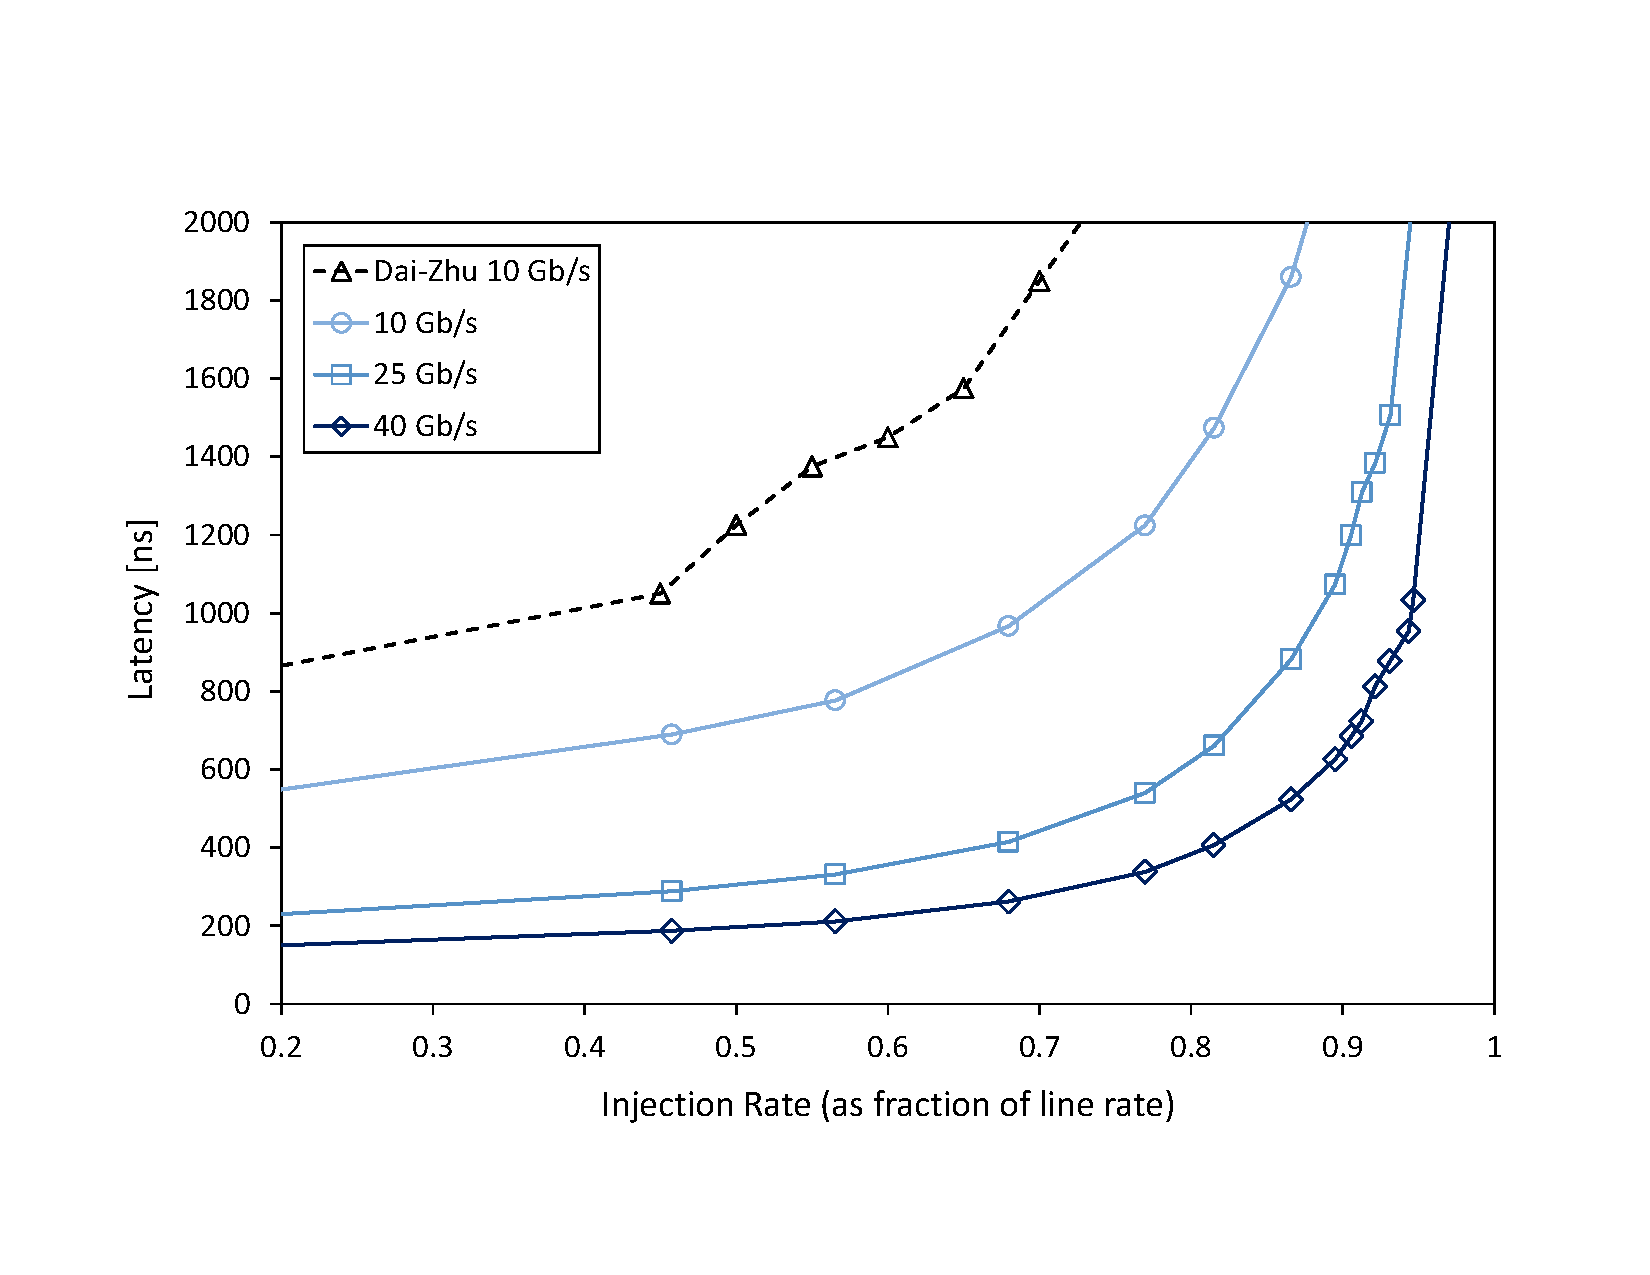
\includegraphics[width=0.485\textwidth, trim = 2cm 2.5cm 2cm 3.4cm, clip]{images/latency-chart-data-320-640.pdf}
\caption{Latency vs. injection rate of the NoC-based Ethernet switch design given line rates of 10, 25, and 40~Gb/s, and compared to the Dai/Zhu 16$\times$16 10~Gb/s FPGA switch fabric design~\cite{dai-zhu}. Our switch queues and Dai/Zhu's switch queues are of size 60kb and 16kb, respectively.}
\label{fig:lat-plot}
\vspace{0cm}
\end{figure}

The average latency of our Ethernet switch design is measured using the \texttt{RTL2Booksim} simulator.
An ON/OFF injection process is used to model bursty, uniform random traffic, with a fixed Ethernet frame size of 512 bytes (as was used in~\cite{dai-zhu}).
Latency is measured as the time between a packet head being injected into the input queue and it arriving out of the output queue.
%The design is simulated at 10, 25, and 40~Gb/s to model modern Ethernet bandwidths, with latency measured and plotted in Fig.~\ref{fig:lat-plot}.
Fig.~\ref{fig:lat-plot} plots the latency of our Ethernet switch at its supported line rates of 10~Gb/s, 25~Gb/s and 40~Gb/s.
Surprisingly, the latency of a 512~byte packet improves at higher line rates.
This is because a higher line rate means a faster rate of injecting NoC flits, and the NoC can handle the extra switching without a large latency penalty thus resulting in an improved overall latency.
%Because the latency of the NoC varies little when the injection bandwidth is below its capacity, NoC-based Ethernet switches of higher throughput inject packets into the NoC at a faster rate and therefore achieve better latency.
No matter what the injection bandwidth, the NoC-based switch considerably outperforms the Dai/Zhu switch~\cite{dai-zhu} for all injection rates.
%The saturation point can be improved by increasing the size of the output queues.
%However, higher throughputs cause the NoC to reach its saturation point at a lower injection rate than lower throughputs.
By supporting these high line rates, our results show that an embedded NoC can push FPGAs into new communication network markets that are currently dominated by ASICs.

%want to say something about programmability being important in these markets, hence the cavium switch.

%Fig.~\ref{fig:lat-plot} plots the latency for both queue depths as a function of the injection rate.
%The ``knee'' in each plot indicates the injection rate at which the output queues become full and start backpressuring the NoC.
%An output queue fills up when it is being driven by multiple sources at the same time, as it can only eject flits at up to the line rate.
%Up until the plot knee, the average latency remains below 65 RTL cycles (156.25 MHz), or 416 ns.

%
\subsection{Packet Processor}



In recent years there has been a surge in demand on computer networks, causing a rapid evolution in network protocols and functionality.
Programmable network hardware has hence become highly desirable~\cite{nunes2014survey,mckeown2008openflow}, as it can provide both the flexibility to evolve and the capacity to support the latest bandwidth demands.
Prior work has demonstrated two ways to implement a flexible and high performing packet processor: the PP packet processor~\cite{attig2011400}, built from an FPGA, and the RMT packet processor~\cite{bosshart2013forwarding}, built from ASIC technology.
Although both provide varying trade-offs between flexibility and performance, we believe a better trade-off can be reached by using a new packet processor design built from the NoC-enhanced FPGA.

Unlike previously proposed programmable packet processors that use an OpenFlow-like cascade of programmable ``flow tables''~\cite{mckeown2008openflow}, our ``NoC Packet Processor'' (NoC-PP~\cite{bitar2015bringing}) uses a modular design style, where various modules are implemented in the FPGA fabric, each dedicated to processing a single network protocol (e.g. Ethernet, IPv4, etc.).
Packets are switched between these protcol processing modules via the embedded NoC.
The flexibility of the FPGA fabric allows the modules to be fully customized and later updated, as existing protocols are enhanced and new protocols are added.
The embedded NoC provides an efficient interconnect that can support switching packets between the modules at modern network bandwidths.

To evaluate this design, we implemented a packet processor that supports processing of several common network protocols: Ethernet, VLAN, IPv4, IPv6, and TCP.
Each packet going through the processor will visit a processing module for each protocol found in its header.
The processing modules are designed with a data path width of 512~bits running at 200~MHz, providing an overall processing throughput of 100~Gb/s.
In order to support higher network bandwidths, several copies of the processing modules are instantiated in the fabric as desired (in this case four instantiations to support 400G, see Figure~\ref{noc-pp-uni}).
%This ability to duplicate individual processing modules, as well as swap them in and out via full/partial reconfiguration provides a key form of design flexibility not found in previously proposed packet processor designs.
Having the generality of the FPGA fabric provides an important advantage to FPGA-based packet processing; whereas the ASIC-based RMT design~\cite{bosshart2013forwarding} provides some flexibility, it is still limited to what is made available upon chip fabrication~\cite{bitar2015bringing}.

We measure the hardware cost and performance of the NoC-PP design and compare it to the PP design~\cite{attig2011400}, another efficient FPGA-based packet processor.
We compare to two versions of the PP design: (1) ``JustEth'', which only performs parsing on the Ethernet header, and (2) ``TcpIp4andIp6'', which performs parsing on Ethernet, IPv4, IPv6 and TCP~\cite{attig2011400}.
Table~\ref{tbl:results} contains hardware cost and performance results of the NoC-PP and PP designs, with hardware cost measured using resource utilization as a percentage of an Altera Stratix V-GS FPGA.
Overall, the NoC-PP proves to be more resource efficient and achieves better performance compared to the PP architecture while providing the same degree of hardware flexibility via the FPGA fabric.
For the smaller application (JustEth), the NoC-PP design is 3.2$\times$ more efficient, whereas for the larger application (TcpIp4Ip6), it is 1.7$\times$ more efficient.
NoC-PP also reduces latency by 3.7$\times$ and 1.5$\times$ compared to PP for JustEth and TcpIp4Ip6, respectively.

\figvs{0.9}{noc-pp-uni}{}{The NoC-PP design for an Ethernet/VLAN/IPv4/IPv6/TCP packet processor (Eth=Ethernet+VLAN). Processing modules run at 100G, and are instantiated four times to support 400G processing.}

\begin{table}[t]
\center
\caption{Comparison of the NoC-PP and PP architectures}
\begin{tabular}{lllll}
\toprule
 \textbf{Application} & \textbf{Architecture} & \textbf{Resource} & \textbf{Latency} & \textbf{Throughput} \\
 & & \textbf{Utilization} & \textbf{(ns)} & \textbf{(Gb/s)} \\
 & & \textbf{(\% FPGA)} & & \\
\midrule
\multirow{2}{*}{JustEth} &  NoC-PP  & 3.6\%  & 79 & 400 \\
                         &  \cellcolor{gray!25}PP~\cite{attig2011400}      & \cellcolor{gray!25}11.6\% & \cellcolor{gray!25}293 & \cellcolor{gray!25}343 \\
\midrule
\multirow{2}{*}{TcpIp4Ip6} &  NoC-PP  & 9.4\%  & 200 & 400 \\
                           &  \cellcolor{gray!25}PP~\cite{attig2011400}      & \cellcolor{gray!25}15.6\% & \cellcolor{gray!25}309 & \cellcolor{gray!25}325 \\
\bottomrule
\end{tabular}
\label{tbl:results}
\end{table}

It is also important to determine what brings these efficiencies to NoC-PP; is it the new module-based packet processor architecture, the introduction of the hard NoC, or a synergistic fusion of the two?
To answer this question, we began by replacing the hard NoC in our design with an equivalent soft NoC, and separately quantified the cost of the NoC and the processing modules.
We also built another iteration of our design using customized soft crossbars such that only modules that need to communicate are connected.
As can be seen in Figure~\mbox{\ref{hard-vs-soft-area}}, the costs of the soft NoC and the soft crossbar are 29$\times$ and 11$\times$ greater than that of the hard NoC, respectively.
The significantly higher cost of building NoC-PP's interconnection network out of the reconfigurable FPGA fabric is due to the fact it runs at a considerably lower clock frequency compared to the hard NoC and must therefore use wide datapaths to transport the high bandwidth data.
Switching between these wide datapaths requires large multiplexers and wide buffers that consume high amounts of resources.
The design therefore achieves significant savings by hardening this interconnect in the embedded NoC.

Since the processing modules form a small fraction of the design cost when using a soft interconnect, NoC-PP can therefore achieve significant overall savings when replacing the soft interconnect with a hard NoC.
On the other hand, the PP design uses a feed-forward design style.
Rather than switching between protocol modules, PP uses tables containing ``microcode'' entries for all possible protocols that must be processed at that stage~\cite{attig2011400}.
Thus, no wide multiplexing exists in the design that can be efficiently replaced by a hard NoC.
The logic and memory within each stage form the majority PP's hardware cost, which would not change if a hard NoC was introduced.
We therefore conclude that the efficiencies from NoC-PP stem from a synergistic fusion of using the hard NoC with our module-based packet processor architecture.

\figvs{1}{hard-vs-soft-area}{}{Area breakdown of NoC-PP when using a hard NoC, a soft NoC or a soft custom crossbar (Xbar).}

%
\subsection{Embedded NoC for FPGA Computing}
\label{sec_pp}

\begin{figure}[t]
\centering
\subfloat[Without NoC.]{
   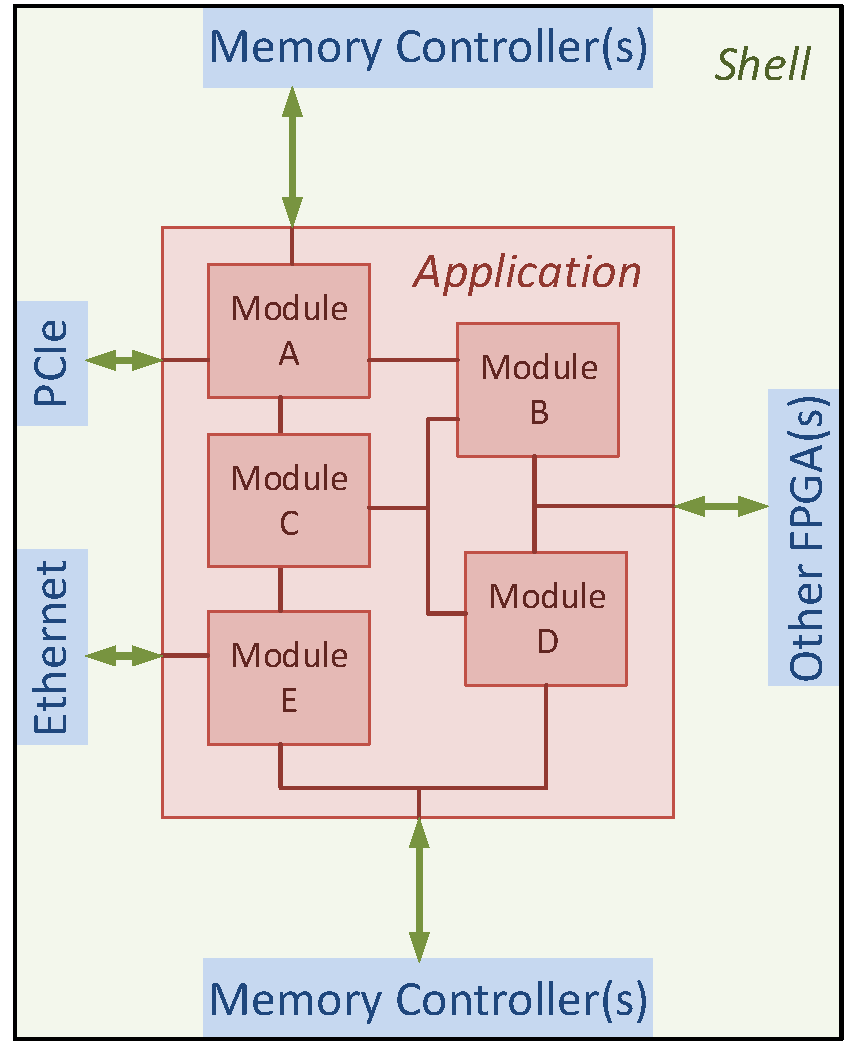
\includegraphics[width=0.5\columnwidth,keepaspectratio]{images/computing}
   \label{computing_no_noc}
 }
\subfloat[With NoC]{
   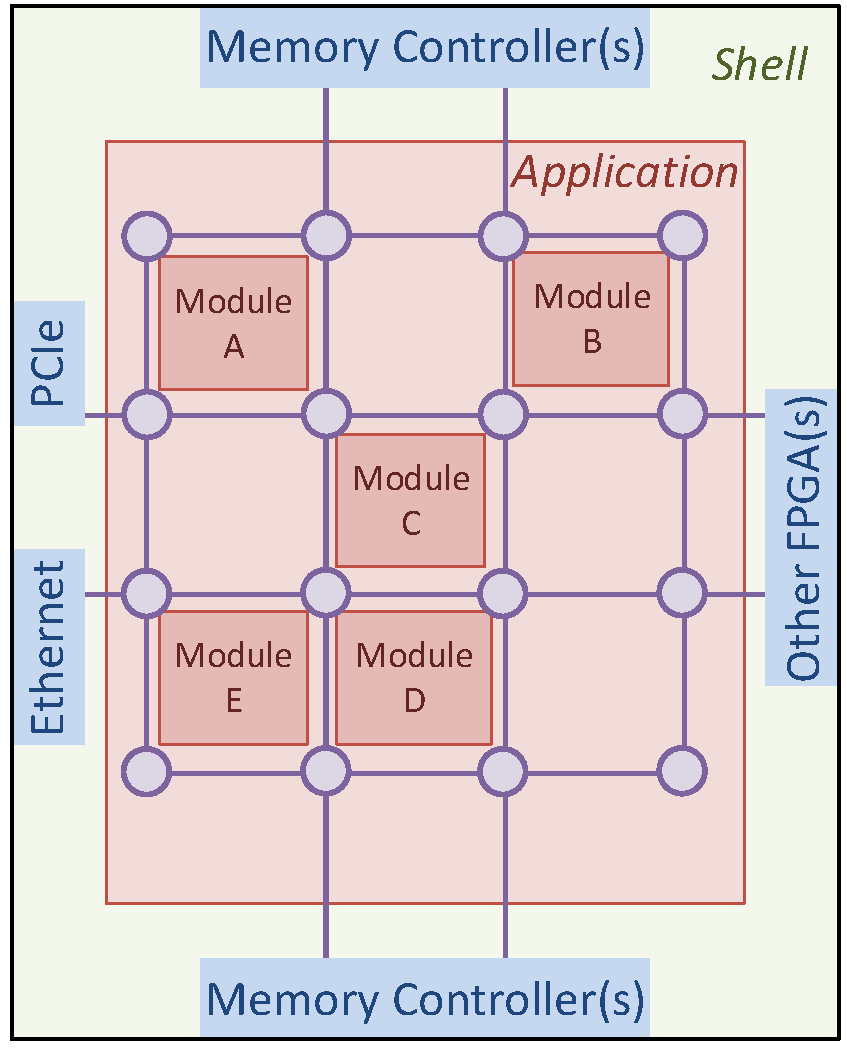
\includegraphics[width=0.5\columnwidth,keepaspectratio]{images/computing_w_noc}
   \label{computing_w_noc}
 }
\caption{A sample FPGA compute accelerator consists of a shell and the application logic.}
\label{computing}
\end{figure}

In this future-looking section, we discuss how an embedded NoC could improve FPGA compute acceleration such as that with data center computing~\cite{Putnam2014} or the OpenCL compute model~\cite{opencl}.
FPGA accelerators consist primarily of two components; the application logic itself, and the \textit{shell} which implements the communication infrastructure for the application.
Fig.~\ref{computing} illustrates the implementation of a compute accelerator, both with and without an embedded NoC.

As Fig.~\ref{computing} shows, a shell consists primarily of a system-level interconnect that connects an application to the host CPU, I/O and memory interfaces, and other FPGAs~\cite{Putnam2014,opencl}.
Built out of soft buses, Microsoft's implementation of this shell occupies approximately one quarter (23\% area) of a large Stratix~V FPGA device~\cite{Putnam2014}.
We believe this area overhead can be reduced if an NoC (with an area of \til1.3\%) is leveraged to interconnect modules in the shell and accelerator -- previous work has already shown that an NoC uses less area and power than soft buses when connecting a system to DDRx memory~\cite{micro}.
Besides the area overhead, it is challenging to meet the timing constraints of the many fast I/O interfaces to which the shell connects -- designers would typically \textit{lock down} the placement and routing of the shell once timing closure is attained, and present standard fixed-location interfaces to the FPGA application logic~\cite{Putnam2014}.
Conversely, an NoC with direct IOLinks to external interfaces can significantly ease timing closure.
Furthermore, any NoC router can be used to connect application modules to the shell instead of fixed-location interfaces -- this would relax the placement and routing constraints of the application and likely improve its performance.
As the JPEG application case study showed, overall application frequency can also be much more predictable with an NoC.
This predictability is especially important when high-level languages (such as OpenCL) are used, and the designer has no direct way to improve operating frequency.

In such compute accelerators, partial reconfiguration is quickly becoming an important feature~\cite{Putnam2014}.
Using partial reconfiguration, the application could either be repaired or replaced without powering down the FPGA, or the data center in which it lies.
To successfully connect a partially reconfigured module, current accelerator shells must provide fixed interfaces and interconnect to the \textit{superset} of the modules that could be partially reconfigured on the FPGA.
This method could be wasteful and complex, and it is often difficult to predict exactly what will be reconfigured in the future.
Instead, we propose using the NoC FabricPorts as a standard, yet flexible interface to partially reconfigured modules.
This avoids the need to explicitly provision a soft bus interface and interconnect for all partially reconfigured modules, since any module connected through a FabricPort will be able to communicate with the rest of the application and I/Os through the embedded NoC.
Our packet processor, NoC-PP in Section~\ref{sec_pp}, could benefit from partial reconfiguration -- the processing modules can be partially reconfigured to update or change the networking protocol.



%\hl{shell construction and using IOLinks to more easily create portable and compatible shells (communication infrastructure).}

%\hl{high-level languages focus on kernels which are then interconnected through a pre-existing NoC. Implementation of things like OpenCL channels. More predictable frequency a big plus for these systems in which the software programmer has no notion of critical path or timing when using the high-level tools}

%\hl{partial reconfiguration in which the NoC can provide a standard interface to which partially-reconfigured modules connect.}

%
%
%#############################################################
\section{Conclusion}
%-0-0-0-0-0-0-0-0-0-0-0-0-0-0-0-0-0-0-0-0-0-0-0-0-0-0-0-0-0-0-
%
%
%

We proposed augmenting FPGAs with an embedded NoC and focused on how to use the NoC for transporting data in FPGA applications of different design styles.
The FabricPort is a flexible interface between the embedded NoC and the FPGA's core; it can bridge any fabric frequency and data width up to 600~bits to the faster but narrower NoC at 1.2~GHz and 150~bits.
We have shown that latency-insensitive systems can be interconnected using an embedded NoC with lower hardware overhead by taking advantage of the NoC's built-in buffering.
Additionally, we showed how latency-sensitive systems can be guaranteed fixed delay and throughput through the NoC by using Permapaths.

We investigated two streaming applications; latency-sensitive JPEG that only requires wires between modules, and a latency-insensitive Ethernet switch that requires heavy arbitration and switching between its transceiver modules.
With an embedded NoC, JPEG's frequency can be improved by 10--80\%\comment{ compared to the FPGA's traditional interconnect with and without pipelining}.
Wire utilization is also improved, as the embedded NoC avoids wiring hotspots and reduces the use of scarce long wires by 40\% at the expense of a 10\% increase of the much more plentiful short wires.
Finally, we showed that high-bandwidth Ethernet switches can be efficiently constructed on the FPGA; by leveraging an embedded NoC we created an 819~Gb/s programmable Ethernet switch -- a major improvement over the 160~Gb/s achieved by prior work in a traditional FPGA.

%
%

%
%
\comment{
%#############################################################
\section*{Acknowledgments}
%-0-0-0-0-0-0-0-0-0-0-0-0-0-0-0-0-0-0-0-0-0-0-0-0-0-0-0-0-0-0-
%
We are indebted to Prof. Natalie Enright-Jerger and her research team for NoC discussions and for providing some of the code used to build \texttt{RTL2Booksim}.
%We would also like to thank David Lewis, Mike Hutton, Dana How and Desh Singh for feedback on FPGAs, and Kevin Murray for feedback on latency-insensitive design.
This work is funded by Altera, NSERC and Vanier CGS.
}


% The very first letter is a 2 line initial drop letter followed
% by the rest of the first word in caps (small caps for compsoc).
%
% form to use if the first word consists of a single letter:
% \IEEEPARstart{A}{demo} file is ....
%
% form to use if you need the single drop letter followed by
% normal text (unknown if ever used by the IEEE):
% \IEEEPARstart{A}{}demo file is ....
%
% Some journals put the first two words in caps:
% \IEEEPARstart{T}{his demo} file is ....
%



% An example of a floating figure using the graphicx package.
% Note that \label must occur AFTER (or within) \caption.
% For figures, \caption should occur after the \includegraphics.
% Note that IEEEtran v1.7 and later has special internal code that
% is designed to preserve the operation of \label within \caption
% even when the captionsoff option is in effect. However, because
% of issues like this, it may be the safest practice to put all your
% \label just after \caption rather than within \caption{}.
%
% Reminder: the "draftcls" or "draftclsnofoot", not "draft", class
% option should be used if it is desired that the figures are to be
% displayed while in draft mode.
%
%\begin{figure}[!t]
%\centering
%\includegraphics[width=2.5in]{myfigure}
% where an .eps filename suffix will be assumed under latex,
% and a .pdf suffix will be assumed for pdflatex; or what has been declared
% via \DeclareGraphicsExtensions.
%\caption{Simulation results for the network.}
%\label{fig_sim}
%\end{figure}

% Note that the IEEE typically puts floats only at the top, even when this
% results in a large percentage of a column being occupied by floats.
% However, the Computer Society has been known to put floats at the bottom.


% An example of a double column floating figure using two subfigures.
% (The subfig.sty package must be loaded for this to work.)
% The subfigure \label commands are set within each subfloat command,
% and the \label for the overall figure must come after \caption.
% \hfil is used as a separator to get equal spacing.
% Watch out that the combined width of all the subfigures on a
% line do not exceed the text width or a line break will occur.
%
%\begin{figure*}[!t]
%\centering
%\subfloat[Case I]{\includegraphics[width=2.5in]{box}%
%\label{fig_first_case}}
%\hfil
%\subfloat[Case II]{\includegraphics[width=2.5in]{box}%
%\label{fig_second_case}}
%\caption{Simulation results for the network.}
%\label{fig_sim}
%\end{figure*}
%
% Note that often IEEE papers with subfigures do not employ subfigure
% captions (using the optional argument to \subfloat[]), but instead will
% reference/describe all of them (a), (b), etc., within the main caption.
% Be aware that for subfig.sty to generate the (a), (b), etc., subfigure
% labels, the optional argument to \subfloat must be present. If a
% subcaption is not desired, just leave its contents blank,
% e.g., \subfloat[].


% An example of a floating table. Note that, for IEEE style tables, the
% \caption command should come BEFORE the table and, given that table
% captions serve much like titles, are usually capitalized except for words
% such as a, an, and, as, at, but, by, for, in, nor, of, on, or, the, to
% and up, which are usually not capitalized unless they are the first or
% last word of the caption. Table text will default to \footnotesize as
% the IEEE normally uses this smaller font for tables.
% The \label must come after \caption as always.
%
%\begin{table}[!t]
%% increase table row spacing, adjust to taste
%\renewcommand{\arraystretch}{1.3}
% if using array.sty, it might be a good idea to tweak the value of
% \extrarowheight as needed to properly center the text within the cells
%\caption{An Example of a Table}
%\label{table_example}
%\centering
%% Some packages, such as MDW tools, offer better commands for making tables
%% than the plain LaTeX2e tabular which is used here.
%\begin{tabular}{|c||c|}
%\hline
%One & Two\\
%\hline
%Three & Four\\
%\hline
%\end{tabular}
%\end{table}


% Note that the IEEE does not put floats in the very first column
% - or typically anywhere on the first page for that matter. Also,
% in-text middle ("here") positioning is typically not used, but it
% is allowed and encouraged for Computer Society conferences (but
% not Computer Society journals). Most IEEE journals/conferences use
% top floats exclusively.
% Note that, LaTeX2e, unlike IEEE journals/conferences, places
% footnotes above bottom floats. This can be corrected via the
% \fnbelowfloat command of the stfloats package.




% if have a single appendix:
%\appendix[Proof of the Zonklar Equations]
% or
%\appendix  % for no appendix heading
% do not use \section anymore after \appendix, only \section*
% is possibly needed

% use appendices with more than one appendix
% then use \section to start each appendix
% you must declare a \section before using any
% \subsection or using \label (\appendices by itself
% starts a section numbered zero.)
%


%\appendices
%\section{Proof of the First Zonklar Equation}
%Appendix one text goes here.

% you can choose not to have a title for an appendix
% if you want by leaving the argument blank
%\section{}
%Appendix two text goes here.


% use section* for acknowledgment
%\ifCLASSOPTIONcompsoc
  % The Computer Society usually uses the plural form
  %\section*{Acknowledgments}
%\else
  % regular IEEE prefers the singular form
  %\section*{Acknowledgment}
%\fi


% Can use something like this to put references on a page
% by themselves when using endfloat and the captionsoff option.
\ifCLASSOPTIONcaptionsoff
  \newpage
\fi



% trigger a \newpage just before the given reference
% number - used to balance the columns on the last page
% adjust value as needed - may need to be readjusted if
% the document is modified later
%\IEEEtriggeratref{8}
% The "triggered" command can be changed if desired:
%\IEEEtriggercmd{\enlargethispage{-5in}}

% references section

% can use a bibliography generated by BibTeX as a .bbl file
% BibTeX documentation can be easily obtained at:
% http://mirror.ctan.org/biblio/bibtex/contrib/doc/
% The IEEEtran BibTeX style support page is at:
% http://www.michaelshell.org/tex/ieeetran/bibtex/
%\bibliographystyle{IEEEtran}
% argument is your BibTeX string definitions and bibliography database(s)
%\bibliography{IEEEabrv,../bib/paper}
%
% <OR> manually copy in the resultant .bbl file
% set second argument of \begin to the number of references
% (used to reserve space for the reference number labels box)
\bibliographystyle{IEEEtran}
\bibliography{IEEEabrv,tcomp}

% biography section
%
% If you have an EPS/PDF photo (graphicx package needed) extra braces are
% needed around the contents of the optional argument to biography to prevent
% the LaTeX parser from getting confused when it sees the complicated
% \includegraphics command within an optional argument. (You could create
% your own custom macro containing the \includegraphics command to make things
% simpler here.)
%\begin{IEEEbiography}[{\includegraphics[width=1in,height=1.25in,clip,keepaspectratio]{mshell}}]{Michael Shell}
% or if you just want to reserve a space for a photo:

\begin{IEEEbiography}[{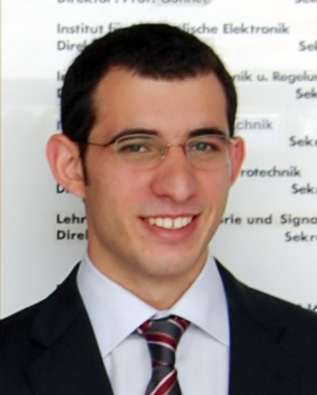
\includegraphics[width=1in,height=1.25in,clip,keepaspectratio]{abdelfattah}}]{Mohamed S. Abdelfattah}
received the BSc degree in ECE from the German University in Cairo in 2009, and the MSc degree in ECE from the University of Stuttgart in 2011.
He is currently pursuing the PhD degree in ECE from the University of Toronto, Canada, where he is researching new communication architectures and CAD tools for FPGAs.
His research interests include FPGA architecture and CAD, on-chip communication, high-level synthesis, and datacenter acceleration.
Mr. Abdelfattah is the recipient of many scholarships and awards, most notably the Vanier Canada Graduate Scholarship and two best paper awards at the FPL 2013 and FPGA 2015 conferences.
\end{IEEEbiography}

% if you will not have a photo at all:
\begin{IEEEbiography}[{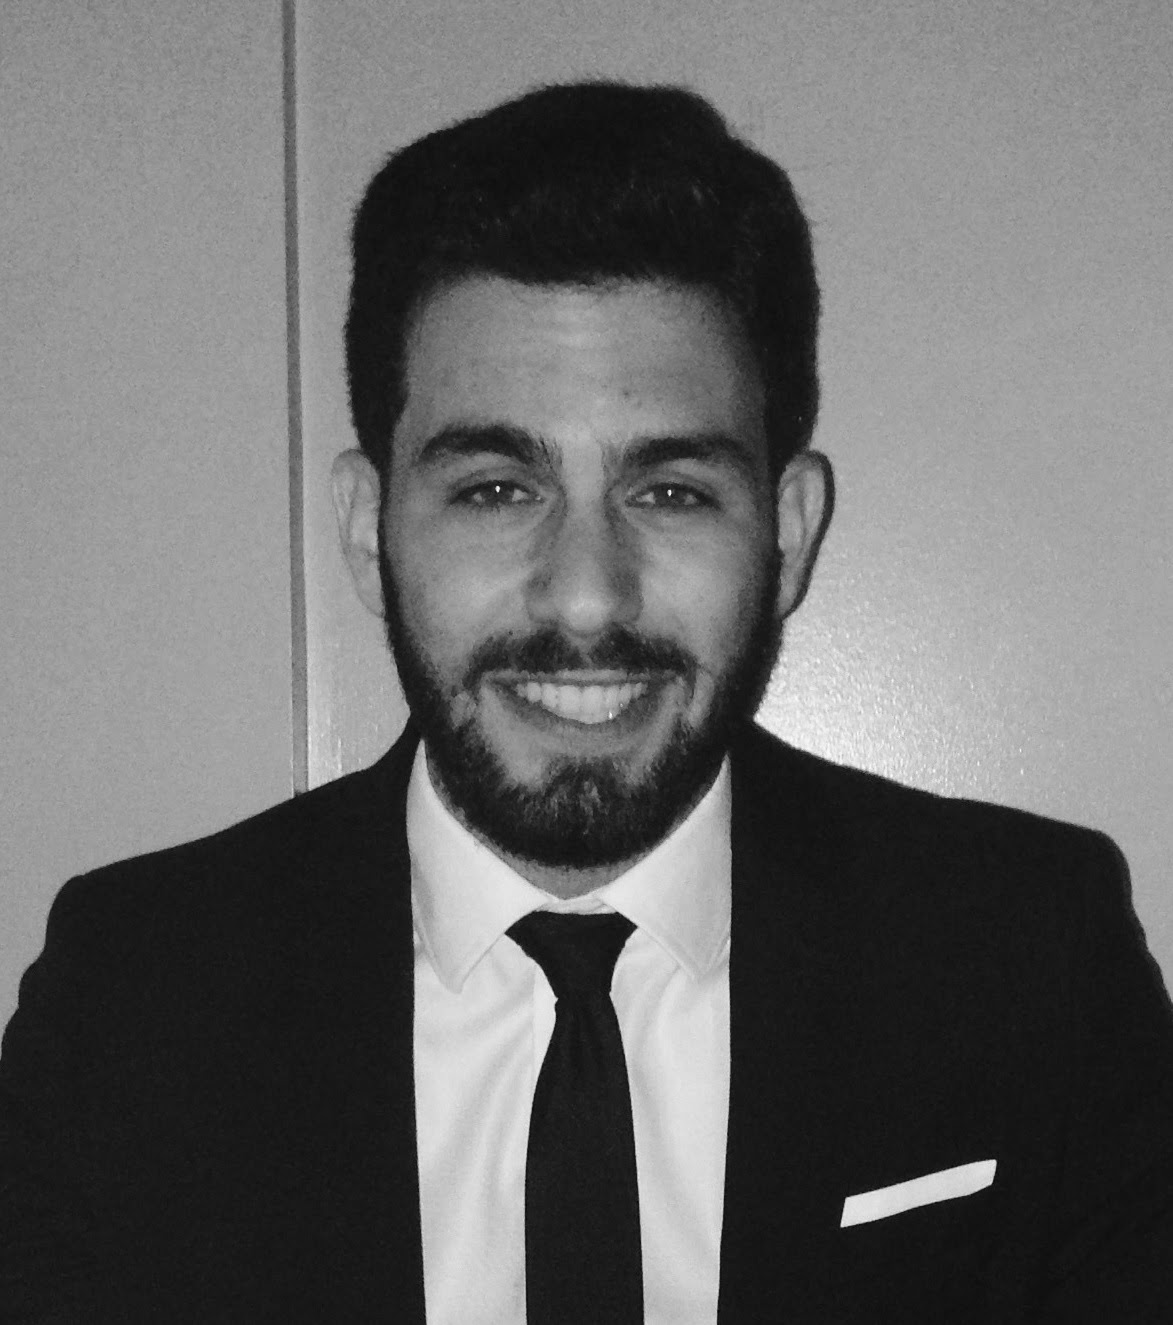
\includegraphics[width=1in,height=1.25in,clip,keepaspectratio]{bitar}}]{Andrew Bitar}
received the BASc degree in ECE from the University of Ottawa in 2013, and the MASc degree in ECE from the University of Toronto in 2015.
His research interests include FPGA acceleration of datacenter and networking applications, as well as high-level synthesis.
Mr. Bitar is the recipient of several scholarships and awards, including the NSERC Canada Graduate Scholarship and the best paper award at the FPGA 2015 conference.
He has been a Design Engineer working on High-Level Design in the Programmable Solutions Group at Intel since 2015.
\end{IEEEbiography}

% insert where needed to balance the two columns on the last page with
% biographies
%\newpage

\begin{IEEEbiography}[{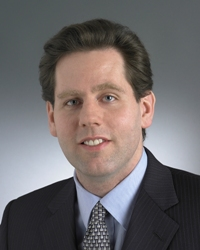
\includegraphics[width=1in,height=1.25in,clip,keepaspectratio]{betz}}]{Vaughn Betz}
received the BSc degree in EE from the University of Manitoba in 1991, the MS degree in ECE from the University of Illinois at Urbana-Champaign in 1993, and the PhD degree in ECE from the University of Toronto in 1998.
Dr. Betz was a co-founder of Right Track CAD in 1998 and its VP of Engineering until its acquisition by Altera in 2000. He held various roles at Altera from 2000 to 2011, ultimately as Senior Director of Software Engineering.
He joined the University of Toronto as an Associate Professor in 2011 and holds the NSERC/Altera Chair in Programmable Silicon; his research covers FPGA architecture, CAD and FPGA-based computation.
\end{IEEEbiography}

% You can push biographies down or up by placing
% a \vfill before or after them. The appropriate
% use of \vfill depends on what kind of text is
% on the last page and whether or not the columns
% are being equalized.

%\vfill

% Can be used to pull up biographies so that the bottom of the last one
% is flush with the other column.
%\enlargethispage{-5in}



% that's all folks
\end{document}
